\documentclass[11pt]{article}
\usepackage[top=2.8cm, bottom=2.8cm, left=2cm, right=2cm]{geometry}
\usepackage{hyperref}
\usepackage{algorithm2e}
\usepackage[numbers]{natbib}
\bibliographystyle{plainnat}
\usepackage{appendix}
\usepackage[table]{xcolor}
\usepackage{pgfplots}
\usepackage{pgfplotstable}
\usepackage[font={color=darkgray,footnotesize, sf, it}]{caption}
\usepackage{amsmath}
\usepackage{helvet}
\usepackage{wrapfig}
\usepackage{anyfontsize}
\usepackage[eulergreek]{sansmath}
\usepackage{listings}
\usepackage{setspace}
\usepackage{graphicx}
\usepackage{longtable}
\usepackage{minted}
\usepackage{relsize}
\usepackage{bchart}
\usepackage{booktabs}
\usepackage{xcolor}
\usepackage{tikz}
\usepackage{collcell}
\usepackage{titlesec}
\linespread{1.2}
\lstset { %
    language=C++,
    backgroundcolor=\color{black!5}, % set backgroundcolor
    basicstyle=\ttfamily\footnotesize,% basic font setting
}

\lstdefinestyle{BashInputStyle}{
  language=bash,
  basicstyle=\footnotesize\ttfamily,
  numbers=left,
  numberstyle=\tiny,
  numbersep=3pt,
  frame=tb,
  columns=fullflexible,
  backgroundcolor=\color{cyan!20},
  linewidth=0.95\linewidth,
  xleftmargin=0.1\linewidth
}

\definecolor{skyblue}{RGB}{203,240,255}
\definecolor{forestgreen}{RGB}{0,96,50}
\definecolor{indigo}{RGB}{4,87,239}
\definecolor{darkindigo}{RGB}{1,40,112}
\definecolor{darkpurple}{RGB}{32,14,104}
\definecolor{apple}{RGB}{0,158,13}
\definecolor{bad}{RGB}{239,55,55}
\definecolor{badtoavg}{RGB}{247,128,98}
\definecolor{avg}{RGB}{255,218,117}
\definecolor{avgtogood}{RGB}{190,247,140}
\definecolor{good}{RGB}{102,226,102}

\setlength{\parindent}{0em}
\setlength{\parskip}{1em}
\setlength\parindent{0pt}
\titlespacing\section{0pt}{12pt plus 4pt minus 2pt}{0pt plus 2pt minus 2pt}
\titlespacing\subsection{0pt}{12pt plus 4pt minus 2pt}{0pt plus 2pt minus 2pt}
\titlespacing\subsubsection{0pt}{12pt plus 4pt minus 2pt}{0pt plus 2pt minus 2pt}

\usepackage{tikz}
\usepackage{collcell}
\usetikzlibrary{shapes.geometric, arrows,calc}
\tikzstyle{startstop} = [rectangle, font=\small, rounded corners, minimum width=4cm, minimum height=0.8cm,text centered, text width=4.5cm, draw=black, fill=gray!50]
\tikzstyle{mpicall} = [rectangle, font=\small, rounded corners, minimum width=4cm, minimum height=0.8cm,text centered, text width=4.5cm, draw=black, fill=cyan!50]
\tikzstyle{mpiproc} = [rectangle, font=\small, minimum width=4.5cm, minimum height=0.8cm, text centered, text width=4.5cm, draw=black, fill=green!60]
\tikzstyle{decision} = [diamond, font=\small, align=center, minimum height=4ex, diamond, aspect=2, text width=14em, inner sep=-1pt, draw=black, fill=violet!50]
\tikzstyle{arrow} = [thick,->,>=stealth]
\tikzstyle{line} = [draw, -latex']

\date{}
\author{}
\title{{\color{indigo}\textbf{CM30225: Parallel Computing}}\\\small \textbf{Distributed Memory Architectures: Balena, MPI and C\\January 2019}\vspace{-15ex}}
\SetKwInOut{Parameter}{parameter}

\begin{document}
\maketitle
\footnotesize\tableofcontents
\clearpage
\normalsize
\pgfplotsset{compat=1.16}

{\color{indigo}
\section{Introduction}}
A \textit{``multiprocessor architecture''} is a broad term applied to parallel architectures involving more than one full processor. A distributed memory architecture is an approach to multiprocessor design which relies on a set of $\mathcal{N}$ processors, each with their own separate memory (and thus separate address spaces) and connected by a common network on which messages can be sent and received between processors.  \textsl{MPI (Message Passing Interface)} is a standard which achieves parallelism on distributed architectures by relying on processes (scheduled on separate cores) communicating with each other via these messages. This is Single Program, Multiple Data (SPMD) parallelism as processes are not in lockstep but are executing the same program.

These messages have an associated cost because network speeds are typically large magnitudes slower than processing speed \citep{nielsen2016}. MPI function calls in code can therefore make it explicit which operations are costly and which are not, unlike alternative approaches such as OpenMP where this cost is somewhat hidden from the programmer.  Due to the messaging overheads, distributed programs are suited to solving very large problems when the overhead is dwarfed by the computation time and parallelism gained. Minimising communication means and keeping data per-process (even if this is means duplication) can therefore reduce runtime compared to lots of messaging overheads for the sake of sharing values.

This assignment requires consideration of the above in implementing matrix relaxation using a distributed memory architecture.

{\color{darkindigo}
\subsection*{Matrix Relaxation}}
Matrix relaxation involves repeatedly replacing a cell's value with the average of its four neighbours (excepting boundary values) until values settle down to a given precision. The task in question was to use C and the OpenMPI library to implement relaxation on a square matrix of dimension $d$, using $n$ MPI processes to a precision of $p$.  The solution was run on \textsl{Balena}, the High Performance Cluster (HPC) at University of Bath\footnote{\url{https://www.bath.ac.uk/corporate-information/balena-hpc-cluster/}} using a variety of configurations to investigate the scalability and correctness of the parallel approach on various problem sizes. As \textsl{Balena} does not allow $n$ to exceed the number of cores available, $n$ will always be less than or equal to this value.

Matrix relaxation holds some inherent sequential properties which require careful synchronisation between processes, as the order of computations is crucial to the output:
\begin{enumerate}
\item \textbf{Consistency of neighbour cells:} For any \textit{inner cell} $c_{i,j}$ (where $i$ is the row and $j$ is the column) to be correctly relaxed, the neighbouring cells ($c_{i+1,j}$, $c_{i-1,j}$, $c_{i,j+1}$, $c_{i,j-1}$) must be kept consistent values throughout the iteration. If any neighbouring cell values were changed (or \textit{relaxed}) between reads for a certain cell, this would cause the value of the cells in the resulting matrix to be incorrect and unpredictable between iterations.  The matrix needs to be divided in such a way without interfering with other processes' computations.
\item \textbf{Precision checks between iterations:} Before a new iteration can start, there needs to be a check across all inner cells as to whether the difference in corresponding matrix values before and after the current iteration is less than or equal to the chosen precision, $p$. There must be careful management over when computation can proceed as processes are not in lockstep.
\end{enumerate}

{\color{indigo} 
\section{Sequential Approach}
\label{sec:seqapproach}}
As presented in coursework 1, the sequential approach can be seen in Algorithm \ref{alg:relaxationsequential}. This relied on working with two matrices of the same dimension $d$ and swapping the references to these after each iteration. This way, the output matrix of iteration $i$ becomes the input to iteration $(i+1)$.  The problem of neighbour cell inconsistency discussed previously is avoided with the introduction of this second (output) matrix. This comes at the cost of an increase in space complexity in memory on the heap, but this is still linear in $d$ which is an appropriate trade off in order to avoid incorrect calculations (new space complexity is $O(2d) = O(d)$, where $d$ is the dimension of the matrix). The fact that swapping input and output matrices comes at the end of each iteration means that no cell can be overwritten with a new relaxed value until every other cell's relaxed value has already been calculated. At step \texttt{9} of Algorithm \ref{alg:relaxationsequential} there is a potentially expensive operation in swapping matrices between every iteration. In order to reduce this overhead, the implementation instead swaps the \textit{references} to each matrix, not the values of each and every inner cell. 

\RestyleAlgo{algoruled}
\LinesNumbered
\DontPrintSemicolon
\SetAlgoLined
\colorbox[gray]{0.95}{
\begin{minipage}{\textwidth}
\begin{algorithm}[H]
  	\caption{Matrix relaxation (sequential).\label{alg:relaxationsequential}}
  	{\color{darkgray}\KwIn{A $d \times d$ matrix with equal fixed edge values and chosen inner values.}
	\KwOut{A $d \times d$ matrix with equal fixed edge values and \textit{\textbf{relaxed}} inner values.}
	\KwData{$d$: Dimension of matrix, $p$: Precision
	}}
	\BlankLine
	{\color{darkgray}Extract program arguments\;
 	Create matrices \texttt{matA} and \texttt{matB} of dimension $d$\;
 	Initialise \texttt{matA} and \texttt{matB} with identical contents\;
 	\BlankLine
 	\Repeat{\texttt{abs(matB[i][j] - matA[i][j])} $\leq p$ for all $(i,j)$}{
		\BlankLine
		\ForEach{inner cell $(i,j)$}
			{\texttt{total $=$ matA[i+1][j]$+$matA[i-1][j]$+$matA[i][j+1]$+$matA[i][j-1]\; matB[i][j] $=$ total $\div$ 4\;}}
 		\BlankLine
 		Swap \texttt{matA} and \texttt{matB}\;
 		}}
\end{algorithm}
\end{minipage}}
\normalsize
\newpage
{\color{indigo}
\section{Parallel Approach}
\label{sec:disapproach}}
Algorithm \ref{alg:relaxationparallel} describes the approach taken in relaxing a matrix using MPI on a distributed architecture. This approach could be described as a weak form of the \textit{master/slave} paradigm. The root process could be seen as a master that is responsible for setting up the main matrix, sending parts of it to and collecting these parts from other processes. However this is where the likeness ends, as each process is still responsible for determining the rows it will read and relax based on its world rank in the communicator. The root process also does some relaxing so is not purely a control process in that respect. The check for whether another iteration is needed is done using a \textit{reduction}, the result of which is sent to every process which provides them with an an awareness of whether to loop again or exit. 

\RestyleAlgo{algoruled}
\LinesNumbered
\DontPrintSemicolon
\SetAlgoLined
\colorbox[gray]{0.95}{
\begin{minipage}{\textwidth}
\begin{algorithm}[H]
  	\caption{Matrix relaxation (parallel).\label{alg:relaxationparallel}}
  	{\color{darkgray}\KwIn{A $d \times d$ matrix with equal fixed edge values and chosen inner values.}
				\KwOut{A $d \times d$ matrix with equal fixed edge values and \textit{\textbf{relaxed}} inner values.}
				\KwData{$d$: Dimension of matrix, $p$: Precision, $n$: Number of MPI processes}}
	\BlankLine
	{\color{darkgray}
	Extract program arguments\;
	Establish connections between $n$ processes\;
	Create main matrix \texttt{m\_main} of dimension $d$\;
	Initialise \texttt{m\_main} with starting values\;
	Distribute $(d-2)$ rows of \texttt{m\_main} between $n$ processes\;
	Create \texttt{m\_read} and \texttt{m\_write} matrices for each process\;
	\BlankLine
	\Repeat{\texttt{next\_iteration\_needed = false}}{
		Scatter assigned rows of \texttt{m\_main} from root to update each process' \texttt{m\_read}\;
		\ForEach{inner cell $(i,j)$ assigned to each process}
			{\texttt{total $=$ m\_read[i+1][j] $+$ m\_read[i-1][j] $+$ m\_read[i][j+1] $+$ m\_read[i][j-1]\; 
			m\_write[i][j] $=$ total $\div$ 4\;}}
			\If{\texttt{abs(m\_read[i][j] - m\_write[i][j])} $> p$ for any $(i,j)$ assigned to current process}{Set \texttt{outside\_prec= true}\;}		
			Gather rows of \texttt{m\_write} from each process to update \texttt{m\_main} on root process\;
 			Set \texttt{next\_iteration\_needed} to reduction (using logical OR) of \texttt{outside\_prec} across all $n$ processes\;	
 		}
 	}
\end{algorithm}
\end{minipage}}

As with any distributed memory implementation using MPI, by attempting to run operations in parallel this way, there are initial overheads in the form of:
\begin{enumerate}
\item \textbf{Management of processes:} Setting up the MPI processes is an overhead in itself\footnote{Making calls such as \texttt{MPI\_Init}, \texttt{MPI\_Comm\_size}, \texttt{MPI\_Comm\_rank} to initialise connections, discover the number of processes running and the current process' rank, then Finalising them all at the end.}. This is a one-off cost which is reduced in my implementation by not making any more calls to create processes at runtime with use of functions such as \texttt{MPI\_Comm\_spawn}. Processes are spawned once at the start of the program and then finalized together once the precision is reached.  If processes were spawned on every iteration the overhead would be substantial (e.g. when $p$ is small, and starting values are a large distance from the converged result causing lots of iterations).
\item \textbf{Management of data:} Allocating each process a certain number of rows to relax in parallel is another overhead. When the problem size is very small this overhead is relatively large, but when the value of $d$ increases this relative cost is reduced. Larger problem sizes (bigger matrices) should reasonably render this initial overhead small compared to the total runtime. Once processes are allocated work to complete, it is important to minimise the messaging overheads required for communication of data between processes - network speeds are a huge bottleneck in the architecture.
\end{enumerate}

{\color{darkindigo}
\subsection*{Dividing the Matrix Between Processes}}
In a similar vein to coursework 1, parallelising the approach to relax the matrix across multiple cores was done with the philosophy of dividing the matrix as evenly as possible. This is because the parallelism gained from all processes having equal work was greater than if one particular task had more work to do, leaving other processes idle before they could be finalised (and introducing some extra unnecessary sequentiality in the process). MPI implementations are SPMD and therefore for a given process $p$ it is impossible to tell if $p$ will finish relaxing the part of the matrix it has been assigned before all other processes, after or somewhere in between.

One crucial difference between the division of work in coursework 1 and this implementation is that the distributed implementation divides the matrix \textit{by whole rows} instead of by individual cells or \textit{sub-divided rows} as before. Whilst dividing by cells (across subdivided or partial rows) could potentially allow greater parallelism with large numbers of processes all doing the same amount of cells, under a distributed memory architecture it would bring with it a lot of unnecessary code complexity and potentially more messaging overheads which renders it not a worthwhile approach - partial rows would require sending extra cells from other partial rows in order to check precision.

This means that for a $d \times d$ matrix being divided across $n$ MPI processes, each process relaxes some of the $(d-2)$ inner rows (initial and final rows of the matrix are initialised to fixed values so do not need relaxing). By splitting the work as equally as possible, then for $n\leq(d-2)$, each process relaxes a base number of $(d-2) \div n$ rows. This is integer division meaning there may in fact be a remaining number of rows unaccounted for if $(d-2) \mod n$ is non-zero (i.e. the number of inner rows does not divide equally by the number of processes). The row remainder is given by $r=(d-2) \mod n$. The value of $r$ is guaranteed to be less than $n$, so the first $r$ processes are given 1 row extra each in order to balance out the row remainder (if any) as fairly and evenly as possible. If $n>(d-2)$ then some processes (those where the rank is greater than $(d-2)$) are allocated 0 rows to relax. This is to prevent subdividing rows and the overheads this would bring. As above, each MPI process is allocated a submatrix (distinct part of the main matrix) to relax. When each process is scheduled it is given its own core to execute the program on which means there is no need to have each process store and update the main matrix. This can be done only by the root process (whose world rank is 0) which means work is not replicated on every core, minimising overheads.

\begin{description}
\item[\textbf{Root process}]: Initialises, stores and updates the main matrix of size $d \times d$. This process scatters a given number of rows to other processes and gathers the relaxed values. It is also responsible for reducing the logical OR operation across all processes' boolean flags in order to determine if the next iteration is needed or whether the main matrix is finally relaxed. Importantly, the root process also does some relaxing itself and it is down to each process itself to work out the part of the matrix it will be relaxing based on its rank, so it is not totally a master/slave approach.
\item[\textbf{Non-root processes}]:  Need a rectangular write-only array of size $r_i \times d$ (where $r_i$ is the number of rows allocated to process $i$ to relax and $d$ is the number of columns in the main matrix). Also need a read-only array of size $(r_{i}+2) \times d$ as each process needs the rows above and below the rows it will relax in order to have enough information available to perform relaxation. As Figure \ref{fig:matreadwrite} shows, the inner values of the row in yellow are relaxed using the values of the rows in green in order to update the non-edge values in the yellow cells. During relaxation, each process has a local copy of a boolean variable which it updates indicating to the root process whether another iteration is necessary (i.e. whether all rows the process has been allocated are relaxed within the given precision $p$). 
\end{description}

\begin{figure}[H]
\centering
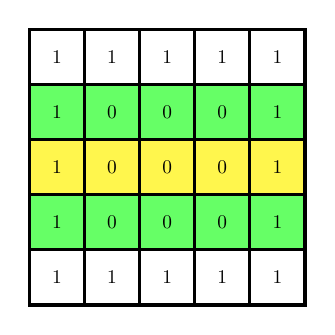
\begin{tikzpicture}
[scale=0.7, writebox/.style={rectangle,draw=black,very thick, minimum size=1cm,scale=0.7},
normbox/.style={rectangle,draw=black,very thick, minimum size=1cm,scale=0.7},
readbox/.style={rectangle,draw=black,very thick, minimum size=1cm,scale=0.7},]
\draw[step=1cm,color=gray,very thick] (0,0) grid (5,5);
\node[normbox] at (0.5,0.5) {1};
\node[normbox] at (1.5,0.5) {1};
\node[normbox] at (2.5,0.5) {1};
\node[normbox] at (3.5,0.5) {1};
\node[normbox] at (4.5,0.5) {1};
\node[readbox,fill=green!60] at (0.5,1.5) {1};
\node[writebox,fill=yellow!70] at (0.5,2.5) {1};
\node[readbox,fill=green!60] at (0.5,3.5) {1};
\node[normbox] at (0.5,4.5) {1};
\node[normbox] at (1.5,4.5) {1};
\node[normbox] at (2.5,4.5) {1};
\node[normbox] at (3.5,4.5) {1};
\node[normbox] at (4.5,4.5) {1};
\node[readbox,fill=green!60] at (4.5,3.5) {1};
\node[writebox,fill=yellow!70] at (4.5,2.5) {1};
\node[readbox,fill=green!60] at (4.5,1.5) {1};

\node[readbox,fill=green!60] at (1.5,1.5) {0};
\node[writebox,fill=yellow!70] at (1.5,2.5) {0};
\node[readbox,fill=green!60] at (1.5,3.5) {0};
\node[readbox,fill=green!60] at (2.5,1.5) {0};
\node[writebox,fill=yellow!70] at (2.5,2.5) {0};
\node[readbox,fill=green!60] at (2.5,3.5) {0};
\node[readbox,fill=green!60] at (3.5,1.5) {0};
\node[writebox,fill=yellow!70] at (3.5,2.5) {0};
\node[readbox,fill=green!60] at (3.5,3.5) {0};
\end{tikzpicture}
\caption{An example $5 \times 5$ matrix. Both green and yellow cells are contained in the read-only matrix of this process. Just the yellow cells are contained in write-only matrix. Only inner yellow values are actually updated.}\label{fig:matreadwrite}
\end{figure}

Memory allocations (for $n\leq(d-2)$ as processes with  $rank>d-2$ are allocated 0 rows) include:
\begin{itemize}
\item The main $d \times d$ matrix initialised once by the root process = $O(d^2)$.
\item The read-only matrix ($2d+ \frac{(d-2)d}{n}$ cells) and write-only matrix ($\frac{(d-2)d}{n}$ cells) on each of the $n$ processes = $O(2d^2)$.
\end{itemize}

This means that as $n$ is a constant, the space complexity is $O(3d^2) \approx O(d^2)$ which is identical to the asymptotic space complexity of the shared memory assignment implementation in coursework 1. 

{\color{darkindigo}
\subsection*{Avoiding Race Conditions}}
A race condition is defined as the consequence of multiple processes reading and writing a shared value with the final result of operations dependent on the order of execution \cite{carr2002}. A data race is a type of race condition which occurs when two or more processes concurrently update a shared value. Each process has a unique block of rows to relax in the overall matrix, but naturally there is some overlap between processes in the rows needed for this computation. In other words, process $x$ will generally need to read a row of the matrix which process $(x-1)$ is relaxing in order to do its own relaxation. Whilst we are now considering a distributed architecture (i.e. separate address spaces so processes can't access the same memory locations), this still requires careful management to avoid data races and synchronise progress across all $n$ processes.

Similar to coursework 1, each process uses two dedicated matrices (one to exclusively read from and one to exclusively write to) during each iteration (Algorithm \ref{alg:relaxationparallel}). Instead of swapping references to these every iteration as in the sequential approach (Algorithm \ref{alg:relaxationsequential}), there is no swapping in this implementation as this is not necessary and (as previously explained) the sizes of the read-only and write-only matrices for each process are different. Instead, each process' read-only matrix is populated by the root process using a call to \texttt{MPI\_Scatterv} and read from many times when rows delegated to this process are relaxed. During each iteration the cells that are read from the read-only matrix are used in relaxation calculations to update the values in the write-only matrix. After a given iteration on each process, a call is made to \texttt{MPI\_Gatherv} to collect values from each write-only matrix and use these to update the main matrix on the root process. 

During a single iteration on each process, several measures mean no data races can occur:
\begin{itemize}
\item Each element of the per-process read-only matrix can be read from any number of times without worrying about other processes updating any of its elements as this memory is not shared (each process has its own address space). 
\item Each element of the per-process write-only matrix is written to once per iteration by a given process. There is no potential for simultaneous read or write operations on the same element of the write-only matrix  as this memory is not shared (each process has its own address space).
\item Calculating the precision (difference between corresponding cells) is a read-only operation done on a per-process basis using its own read-only and write-only matrices which are not shared locations in memory (each process has its own address space).
\item MPI calls to scatter and gather values from each process' matrices are \textit{blocking} - a global precision check across all processes is done on the root process in a synchronised fashion. No process can start a new iteration before the previous one has finished.
\end{itemize}

There is extra space complexity in the approach of each process containing 2 matrices (comprising of parts of the main matrix) but this is more desirable than broadcasting the entire matrix of values to each process, requiring extra messaging overheads between processes.

{\color{darkindigo}
\subsection*{Dealing with Messaging Overheads}}
Another important (arguably the most crucial) consideration here was reducing the number (and size of) messages required for processes to do their work. As in the introduction, this transfer of data between processors using the network bus is substantially slower than making data accesses on the same node or processor cache.

An extremely inefficient and poorly-scalable solution might use \texttt{MPI\_Bcast} in order to perform a broadcast of the entire main matrix from the root process to each of the other processes in the world communicator so they have their own copy to work with. However, using a broadcast makes the total messaging overhead unnecessarily large. If a $5000 \times 5000$ matrix of \texttt{double} values (8 bytes) is to be broadcast across 64 processes running across 4 nodes that requires $8 \times 5000 \times 5000 = 200$MB to be broadcast to each of 64 processes (12.8GB total) - this is where the lack of scalability becomes obvious. Every process does not need to have knowledge of how the overall matrix looks so this approach was decided against. Instead, using the same example, \texttt{MPI\_Scatterv} sends around $8 \times (2 \times 5000 + \frac{(5000-2) \times 5000}{64}) = 3.2$MB to each process (0.2GB total).

Messages are asynchronous, but some MPI calls such as \texttt{MPI\_Scatterv} and \texttt{MPI\_Gatherv} are are \textit{blocking} which means processes will wait until they all reach the call before continuing. Again this brings with it a speed cost but is necessary for correct operation and synchronisation between processes before continuing to the next iteration.  The main MPI calls used in the implementation are displayed below to illustrate how the implementation scatters and gathers rows of the main matrix between the different MPI processes and how they send back to the root their updated cell values when they are finished. In order to understand when the program can terminate, a logical OR reduction operation is used to check that each process does or does not need another iteration before their work is done.

\hspace{-0.5cm}\begin{minipage}[t]{0.4\textwidth}
  \centering\raisebox{\dimexpr \topskip-\height}{%
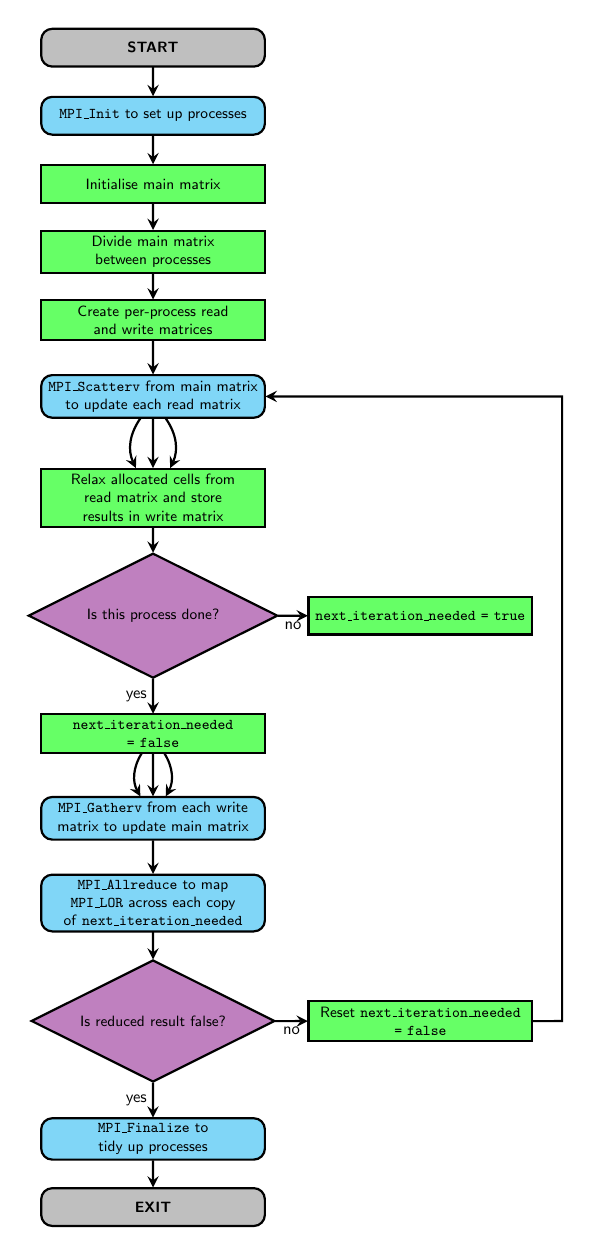
\begin{tikzpicture}[node distance=4.1em,thick,scale=0.6, every node/.style={scale=0.6}]
\node (start) [startstop] {\textsf{\textbf{START}}};
\node (setupmpi) [mpicall, below of=start] {\texttt{MPI\_Init} \textsf{to set up processes}};
\node (initmat) [mpiproc, below of=setupmpi] {\textsf{Initialise main matrix}};
\node (dividework) [mpiproc, below of=initmat] {\textsf{Divide main matrix between processes}};
\node (createarrays) [mpiproc, below of=dividework] {\textsf{Create per-process read and write matrices}};
\node (scatterv) [mpicall, below of=createarrays, yshift=-0.5em] {\texttt{MPI\_Scatterv} \textsf{from main matrix to update each read matrix}};
\node (relax) [mpiproc, below of=scatterv, yshift=-2em] {\textsf{Relax allocated cells from read matrix and store results in write matrix}};
\node (preccheck1) [decision, below of=relax, yshift=-3em] {\textsf{Is this process done?}};
\node (setflagtrue)  [mpiproc, right of=preccheck1, xshift=12em] {\texttt{next\_iteration\_needed = true}};
\node (setflagfalse)  [mpiproc, below of=preccheck1, yshift=-3em] {\texttt{next\_iteration\_needed = false}};
\node (gatherv) [mpicall, below of=setflagfalse, yshift=-1em] {\texttt{MPI\_Gatherv} \textsf{from each write matrix to update main matrix}};
\node (allreduce) [mpicall, below of=gatherv, yshift=-1em] {\texttt{MPI\_Allreduce} \textsf{to map} \texttt{MPI\_LOR} \textsf{across each copy of} \texttt{next\_iteration\_needed}};
\node (preccheck2) [decision, below of=allreduce, yshift=-3em] {\textsf{Is reduced result false?}};
\node (resetflag)  [mpiproc, right of=preccheck2, xshift=12em] {\textsf{Reset} \texttt{next\_iteration\_needed = false}};
\node (finalizempi) [mpicall, below of=preccheck2, yshift=-3em] {\texttt{MPI\_Finalize} \textsf{to tidy up processes}};
\node (end) [startstop, below of=finalizempi] {\textsf{\textbf{EXIT}}};

\draw [arrow] (start) -- (setupmpi);
\draw [arrow] (setupmpi) -- (initmat);
\draw [arrow] (initmat) -- (dividework);
\draw [arrow] (dividework) -- (createarrays);
\draw [arrow] (createarrays) -- (scatterv);
\draw [arrow, bend left] (scatterv) edge (relax);
\draw [arrow] (scatterv) -- (relax);
\draw [arrow, bend right] (scatterv) edge (relax);
\draw [arrow] (relax) -- (preccheck1);
\draw [arrow] (preccheck1) -- node[anchor=north] {\textsf{no}} (setflagtrue);
\draw [arrow] (preccheck1) -- node[anchor=east] {\textsf{yes}} (setflagfalse);
\draw [arrow, bend left] (setflagfalse) edge (gatherv);
\draw [arrow] (setflagfalse) -- (gatherv);
\draw [arrow, bend right] (setflagfalse) edge (gatherv);
\draw [arrow] (gatherv) -- (allreduce);
\draw [arrow] (allreduce) -- (preccheck2);
\draw [arrow] (preccheck2) -- node[anchor=north] {\textsf{no}} (resetflag);
\draw [arrow] (preccheck2) -- node[anchor=east] {\textsf{yes}} (finalizempi);
\draw [arrow] (resetflag) -- ++(3,0) |- (scatterv);
\draw [arrow] (finalizempi) -- (end);
\end{tikzpicture}}
        \captionof{figure}{Diagram of the overall execution life cycle.}
        \label{fig:mpicalls}
\end{minipage}\hspace{1.5cm}
\begin{minipage}[t]{0.55\textwidth}
The program relies on the following MPI calls (shown in Figure \ref{fig:mpicalls}):
\begin{description}
\item[\texttt{MPI\_Init}, \texttt{MPI\_Comm\_size}, \texttt{MPI\_Comm\_rank}]: First, the connections between processes are initialised and the size of the communicator is determined so that the matrix can be divided between the $n$ processes. It is useful to determine the rank of the current process to allow different parts of the matrix to be allocated based on the current process rank.
\item[\texttt{MPI\_Scatterv}] This is \textit{blocking}. $2d+ \frac{(d-2)d}{n}$ cells are sent from the root process to update each process' read-only matrix with values. From here, cells can be read from each process' copy of the read-only matrix to relax the values and store results in the process' write-only matrix. \texttt{MPI\_Scatter} requires chunks of equal size to be sent to each process, so in the case of unequal division of work, \texttt{MPI\_Scatterv} is more suitable.
\item[\texttt{MPI\_Gatherv}] This is \textit{blocking}. $\frac{(d-2)d}{n}$ cells are collected from each process write-only matrix to update the main matrix on the root process. \texttt{MPI\_Gather} requires chunks of equal size to be gathered from each process, so in the case of unequal division of work, \texttt{MPI\_Gatherv} is more suitable.
\item[\texttt{MPI\_Allreduce}] This is \textit{blocking}. A logical OR operation is reduced across all $n$ processes to determine if a new iteration is needed. An alternative would be for processes to use an \texttt{MPI\_Bcast} to inform other processes whether they need another iteration, but this introduces extra unnecessary messaging overheads. Any \texttt{true} value from any of the processes indicates another iteration is needed, as this makes the result of \texttt{MPI\_LOR} \texttt{true} as well.
\item[\texttt{MPI\_Finalize}] This is \textit{blocking}. A necessary call is made to terminate all MPI processes before the program exits.
\end{description}
\end{minipage}

{\color{darkindigo}
\subsection*{Precision Checks}}
During each iteration each process writes to its own local copy of a boolean flag \texttt{next\_iteration\_needed} if any of the differences in values before and after relaxation of a given cell fall outside the prevision window defined by $p$. In order to determine when relaxation has finished across all processes, the (synchronising) call to \texttt{MPI\_Allreduce} is made with the \texttt{MPI\_LOR} operation at the end of each iteration which aggregates all values of \texttt{next\_iteration\_needed} into one single boolean \texttt{outside\_prec}. If this is false, we can break from the relaxation loop and print the final matrix. If this is true then that is because one of the processes needs at least 1 more iteration before it is relaxed, so we loop again and scatter newly updated values to each process' read-only matrix for the next iteration of relaxation to begin.

It is not entirely clear how much latency this blocking call to \texttt{MPI\_Allreduce} adds to the overall runtime but it is ncessary to synchronise processes in understanding whether another iteration is needed before they can continue. Non-blocking MPI calls such as \texttt{MPI\_Isend} might cause less latency here, but cause code to be more complex when synchronising the decision over whether to continue to the next iteration.  Simply calling \texttt{MPI\_Reduce} instead of \texttt{MPI\_Allreduce} would mean that the aggregated result of the operation would not be broadcasted to each process (the result would just be available to the root), so each couldn't check the result of \texttt{outside\_prec} and exit accordingly. The approach aims to achieve a ``superstep'' model of computation (Figure \ref{fig:superstep}). Processes work on their own section of the main matrix during each iteration, with a certain amount of sequentiality necessary when they are synchronised at the end of an iteration to check if we need to continue to the next.

\begin{figure}[H]
\centering
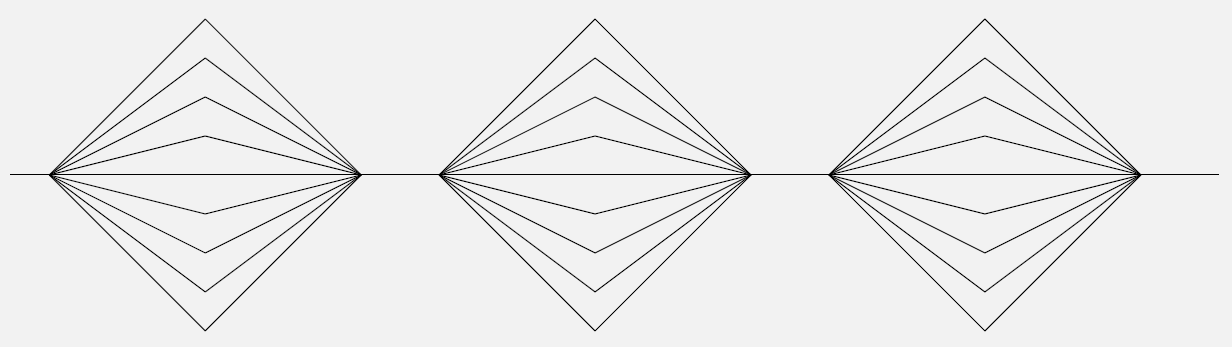
\includegraphics[scale=0.2]{img/superstep.png} 
\caption{Diagram showing the ``superstep programming'' method with \texttt{MPI\_Scatterv} and \texttt{MPI\_Gatherv}.}\label{fig:superstep}
\end{figure}

{\color{darkindigo}
\subsection*{Storage and Indexing of the Matrices}}
By storing the overall matrix and smaller read/write matrices for each process as a 1D arrays, it does mean there must exist a mechanism for indexing and checking if we are inspecting an edge cell when relaxing. This is a definite overhead in the implementation, however  MPI calls expect that memory storing values to be sent to other processes is contiguous, which is only true for a given row of a 2D array. In the shared memory implementation, the 2D array was actually a 1D array of pointers to 1D arrays. This does not translate into distributed architectures as one processor's address space is not accessible by another process using pointers - trying to send or broadcast pointers to processes is nonsensical. Making a deep copy of rows to be sent would be even more costly than an indexing mechanism, so this approach isn't feasible. As such, a 1D array is used to store the main matrix in a continuous block and allow easier partitioning and sending of data to other processes.

{\color{darkindigo}
\subsection*{Choice of Initial Matrix Values}}
In the shared memory coursework, whilst edge cells were fixed to a value of 1.0, inner cells were initialised using random numbers which required thought over reproducibility during testing stages. It made timings (even using the same seed) harder to interpret and required running several tests before calculating an average. Random initial inner values might take a variable amount of time to relax across sizes purely because of their values being (by chance) further away from the final relaxed values. In light of feedback received, the initial values of the matrix are now set to a \textit{fixed non-random pattern}.  Values are now initialised to 0.0 on the inner cells, with 1.0 remaining as the value of edge cells. This gives better reproducibility during timings and allows more meaningful comparisons to be made across matrix sizes. 

{\color{indigo}
\section{Testing Program Correctness}}
In order to verify whether the approach taken was correct, it required a combination of manual verification and a set of varied test cases, where input and output were compared for correctness. See Appendix \ref{apdx:runprog} for how to run the implementation with different configurations.

{\color{darkindigo}
\subsection*{Manual Verification}}
The first stage in testing program correctness was to check against a manually-calculated matrix relaxation in order to check that the parallel C implementation finished after an equal number of iterations and contained equal cell values to the manually-calculated relaxed matrix. \textbf{In the implementation, the main matrix is represented as a 1D array. Rows and columns are indexed from 0}. This means indices 0-4 references the first row, indices 5-9 represents seconds row and so on. 

The relaxation process was executed by hand on the below $5 \times 5$ matrix using the following arguments: $d = 5$, $p = 0.2$, $n = 3$.  Using the parallel algorithm shown in Algorithm \ref{alg:relaxationparallel}, the $(d-2) = 3$ inner rows are divided equally across the 3 processes. Between iterations, the maximum difference in cell values ($\max(|c_{new}-c_{old}|)$) for each process was calculated, to check if this was within the desired precision of $p = 0.2$. 

\textbf{Each process first determines its part of the matrix to read and relax:}
\begin{description}
\item[\textbf{Process 1}]: Root scatters cells 0-14 (rows 0-2 inclusive to read) and gathers cells 5-9 (row 1 relaxed).
\item[\textbf{Process 2}]: Root scatters cells 5-19 (rows 1-3 inclusive to read) and gathers cells 10-4 (row 2 relaxed).
\item[\textbf{Process 3}]: Root scatters cells 10-24 (rows 2-4 inclusive to read) and gathers cells 15-19 (row 3 relaxed).
\end{description}

The manual calculation was as follows:

\hspace{-0.2cm}\begin{minipage}{0.47\textwidth}
$
\begin{bmatrix}
1.000000 & 1.000000 & 1.000000 & 1.000000 & 1.000000 \\
1.000000 & 0.000000 & 0.000000 & 0.000000 & 1.000000 \\
1.000000 & 0.000000 & 0.000000 & 0.000000 & 1.000000 \\
1.000000 & 0.000000 & 0.000000 & 0.000000 & 1.000000 \\
1.000000 & 1.000000 & 1.000000 & 1.000000 & 1.000000 \\
\end{bmatrix}
$
\end{minipage}\hspace{1.8cm}{\color{cyan!90}\vline}\hspace{0.5cm}
\begin{minipage}{.47\textwidth}
\vspace{-1em}
\textbf{Initial Matrix:} The matrix of \texttt{double} values is set to a fixed non-random pattern: $1.000000$ on the edges, and $0.000000$ on the inner cells. We scatter this in sections as described above to each process.
\vspace{-1em}
\end{minipage}

\hspace{-0.2cm}\begin{minipage}{0.47\textwidth}
$
\begin{bmatrix}
1.000000 & 1.000000 & 1.000000 & 1.000000 & 1.000000 \\
1.000000 & 0.500000 & 0.250000 & 0.500000 & 1.000000 \\
1.000000 & 0.250000 & 0.000000 & 0.250000 & 1.000000 \\
1.000000 & 0.500000 & 0.250000 & 0.500000 & 1.000000 \\
1.000000 & 1.000000 & 1.000000 & 1.000000 & 1.000000 \\
\end{bmatrix}
$
\end{minipage}\hspace{1.8cm}{\color{cyan!90}\vline}\hspace{0.5cm}
\begin{minipage}{.47\textwidth}\textbf{Iteration 1:}\\
A relaxed submatrix from each processes is gathered by the root to update the main matrix. Global precision isn't reached just yet.
\\
\\
\begin{tabular}{|c|c|c|}
\hline
\textbf{Process} & \textbf{$\max(|c_{new}-c_{old}|)$} & \textbf{$\leq p$?} \\
\hline
\texttt{1} & $|0.000000-0.250000|$ & {\color{red}\texttt{false}}\\
\texttt{2} & $|0.000000-0.250000|$ & {\color{red}\texttt{false}}\\
\texttt{3} & $|0.000000-0.250000|$ & {\color{red}\texttt{false}}\\
\hline
\end{tabular}
\end{minipage}

\hspace{-0.4cm}\begin{minipage}{0.47\textwidth}
$
\begin{bmatrix}
1.000000 & 1.000000 & 1.000000 & 1.000000 & 1.000000 \\
1.000000 & 0.625000 & 0.500000 & 0.625000 & 1.000000 \\
1.000000 & 0.500000 & 0.250000 & 0.500000 & 1.000000 \\
1.000000 & 0.625000 & 0.500000 & 0.625000 & 1.000000 \\
1.000000 & 1.000000 & 1.000000 & 1.000000 & 1.000000 \\
\end{bmatrix}
$
\end{minipage}\hspace{1.8cm}{\color{cyan!90}\vline}\hspace{0.5cm}
\begin{minipage}{.47\textwidth}\textbf{Iteration 2:}\\
A relaxed submatrix from each processes is gathered by the root to update the main matrix. Global precision isn't reached just yet.
\\
\\
\begin{tabular}{|c|c|c|}
\hline
\textbf{Process} & \textbf{$\max(|c_{new}-c_{old}|)$} & \textbf{$\leq p$?} \\
\hline
\texttt{1} & $|0.500000-0.250000|$ & {\color{red}\texttt{false}}\\
\texttt{2} & $|0.500000-0.250000|$ & {\color{red}\texttt{false}}\\
\texttt{3} & $|0.500000-0.250000|$ & {\color{red}\texttt{false}}\\
\hline
\end{tabular}
\end{minipage}

\hspace{-0.4cm}\begin{minipage}{0.47\textwidth}
$
\begin{bmatrix}
1.000000 & 1.000000 & 1.000000 & 1.000000 & 1.000000 \\
1.000000 & 0.750000 & 0.625000 & 0.750000 & 1.000000 \\
1.000000 & 0.625000 & 0.500000 & 0.625000 & 1.000000 \\
1.000000 & 0.750000 & 0.625000 & 0.750000 & 1.000000 \\
1.000000 & 1.000000 & 1.000000 & 1.000000 & 1.000000 \\
\end{bmatrix}
$
\end{minipage}\hspace{1.8cm}{\color{cyan!90}\vline}\hspace{0.5cm}
\begin{minipage}{.47\textwidth}\textbf{Iteration 3:}\\
A relaxed submatrix from each processes is gathered by the root to update the main matrix. Global precision isn't reached just yet.
\\
\\
\begin{tabular}{|c|c|c|}
\hline
\textbf{Process} & \textbf{$\max(|c_{new}-c_{old}|)$} & \textbf{$\leq p$?} \\
\hline
\texttt{1} & $|0.750000-0.625000|$ & {\color{blue}\texttt{true}}\\
\texttt{2} & $|0.500000-0.250000|$ & {\color{red}\texttt{false}}\\
\texttt{3} & $|0.750000-0.625000|$ & {\color{blue}\texttt{true}}\\
\hline
\end{tabular}
\end{minipage}

\hspace{-0.4cm}\begin{minipage}{0.47\textwidth}
$
\begin{bmatrix}
1.000000 & 1.000000 & 1.000000 & 1.000000 & 1.000000 \\
1.000000 & 0.812500 & 0.750000 & 0.812500 & 1.000000 \\
1.000000 & 0.750000 & 0.625000 & 0.750000 & 1.000000 \\
1.000000 & 0.812500 & 0.750000 & 0.812500 & 1.000000 \\
1.000000 & 1.000000 & 1.000000 & 1.000000 & 1.000000 \\
\end{bmatrix}
$
\end{minipage}\hspace{1.8cm}{\color{cyan!90}\vline}\hspace{0.5cm}
\begin{minipage}{.47\textwidth}\textbf{Relaxed Matrix (4 iterations):}\\
A relaxed submatrix from each processes is gathered by the root to update the main matrix. Global precision is reached so we can exit.
\\
\\
\begin{tabular}{|c|c|c|}
\hline
\textbf{Process} & \textbf{$\max(|c_{new}-c_{old}|)$} & \textbf{$\leq p$?} \\
\hline
\texttt{1} & $|0.750000-0.625000|$ & {\color{blue}\texttt{true}}\\
\texttt{2} & $|0.625000-0.500000|$ & {\color{blue}\texttt{true}}\\
\texttt{3} & $|0.750000-0.625000|$ & {\color{blue}\texttt{true}}\\
\hline
\end{tabular}
\end{minipage}

This step-by-step manual calculation shows checks for precision across each process' rows after they have been relaxed and gathered, which is used to decide whether another iteration is needed.  Once the manual calculation had taken place, I populated the initial matrix with identical values and ran the distributed program on \textsl{Balena} to compare outputs:
\begin{lstlisting}[style=BashInputStyle]
	#SBATCH --nodes=1
	#SBATCH --ntasks-per-node=3
    mpirun -np 3 ./distributedrelax -d 5 -p 0.2 -v
\end{lstlisting}
The resulting output included:
\begin{lstlisting}[style=BashInputStyle]
	INFO: MPI proc #0 allocated 1 row(s) of matrix to relax (starts 1 row(s) from top).
	INFO: MPI proc #1 allocated 1 row(s) of matrix to relax (starts 2 row(s) from top).
	INFO: MPI proc #2 allocated 1 row(s) of matrix to relax (starts 3 row(s) from top).
	...
	INFO: 3 processes running...
	...
	INFO: ___Relaxed Matrix (4 iterations)_______
	1.000000 1.000000 1.000000 1.000000 1.000000
	1.000000 0.812500 0.750000 0.812500 1.000000
	1.000000 0.750000 0.625000 0.750000 1.000000
	1.000000 0.812500 0.750000 0.812500 1.000000
	1.000000 1.000000 1.000000 1.000000 1.000000
\end{lstlisting}

Upon observing that that the parallel C implementation matched the manual example at each step, I varied the value of \texttt{-np} from 1 to 12 (running 1-3 processes across 1-4 nodes). Outputs from these tests were saved to files and compared using the Unix \texttt{diff} tool to verify that the total number of iterations required and the matrix values at each stage were identical, which was a success. These outputs are visible in the \texttt{tests} directory of this submission (e.g. the file \texttt{manual\_correctness\_N=1\_TPN=3\_output.txt} is the output of running the program on 1 node with 3 tasks per node). The manual verification stage was then performed on a variety of other small ($d\leq 6, n\leq 5$) examples, with values compared to the result of the sequential and parallel implementations. This made me confident that for small matrices with a small number of processes, the result of the computation could be trusted as correct. 

{\color{darkindigo}
\subsection*{Automated Test Cases}}
For tests with larger matrices and more processes involved, I was not as confident because scaling the problem or splitting it across more processes could indeed expose more problems that weren't as detectable on small examples. For this reason, I went on to produce automated tests where the number of iterations and values of matrix cells at each iteration could be compared at larger scales. 

In order to verify the program's correctness in a more automated sense at larger scale, I created a short test script to compare outputs when running the program under different configurations on increasingly large matrices. I modified the program to only print the state of the matrix after each iteration, as well as the number of iterations it took to relax the matrix, using the \texttt{-i} argument for ``information mode''. This full test script is viewable in Appendix \ref{apdx:correctnesstest}. Its output is saved to a file in the \texttt{tests} directory of this submission (\texttt{automated\_correctness\_full\_output.txt}). 

\begin{lstlisting}[style=BashInputStyle]
    $		./correctness_test.bash
\end{lstlisting}

This script computed the matrix for a given dimension $d$ using 1 MPI process ($n=1$), then compared this output to the result of running under the same conditions with increasing numbers of processes ($n=\{2,...,50\}$).  This was then repeated for increasingly large matrices ($d=\{10,...,2000\}$).  As initial matrix inner cell values are all set to 0, this was kept the same during correctness testing in all trials of each matrix at size $d$, to produce consistent and reproducible results. To ensure each test case was reproducible, I also ensured each was run 25 times to account for potential race conditions occurring that can go undetected if a test was only run once.  It must be noted that whilst all tests passed after 25 repetitions and no bugs or race conditions were detected, this does not guarantee or prove full program correctness. For extra assurance, the output of the parallel implementation for these configurations were compared using the \texttt{diff} tool to the sequential implementation's output which also showed no difference in matrix values at each iteration.

Whilst the test cases are not fully exhaustive, nor guaranteed to show full program correctness in themselves, they do provide greater confidence in the program producing correct and consistent output and handling race conditions at these scales. Combined with the successful manual verification to check for correctness on smaller examples, and the consistency in these outputs seen with larger matrices and numbers of MPI processes, the program can be regarded as producing correct outputs within the context of this assignment. \textbf{Full results are detailed in Appendix \ref{apdx:autocorrtests}.} 

\newpage
{\color{indigo}
\section{Scalability Investigation}}
After the manual and automated correctness testing stage, experiments were performed to understand how scalable the parallel implementation was using \textsl{Balena}, under different program configurations.  The \texttt{real} value given by the Unix \texttt{time} command was used to measure execution time, with the values of the \textsl{SLURM} job script listed below being modified to change the number of nodes and tasks (processes) per node used. For example, the below will execute 6 MPI processes across 3 nodes (2 per node), all relaxing a $25000 \times 25000$ matrix to a precision of $0.01$:
\begin{lstlisting}[style=BashInputStyle]
	#SBATCH --nodes=3
	#SBATCH --ntasks-per-node=2
	time mpirun -np $SLURM_NTASKS ./distributedrelax -d 25000 -p 0.01
\end{lstlisting}

\textsl{Balena} does not allow the value of the \texttt{-np} flag to be set to more than the number of cores available and as such, the value used for \texttt{-np} in scalability tests was bound between 1 (1 node executing 1 process) and 64 (4 nodes executing 16 processes each). \textbf{Full results of testing can be seen in Appendix \ref{apdx:testresults}}. 

{\color{darkindigo}
\subsection*{Comments on Reproducibility and Speedup}}
Some uncontrollable factors can affect the runtime of the problem, including the distance of values from a converged result. Because of this, as mentioned above, initial values of the matrix are now set to a \textit{fixed non-random pattern} of 0.0 on the inner cells, with 1.0 on edge cells. This gives better reproducibility during timings and allows more meaningful comparisons to be made across matrix sizes. 

In the following experiments, \textbf{speedup calculations use the time for $n=1$ as the ``sequential'' execution time}. The reason for this is because by changing the original sequential algorithm (Algorithm \ref{alg:relaxationsequential}) to run in parallel, it has fundamentally changed the way the algorithm operates (by dividing work etc. - see Algorithm \ref{alg:relaxationparallel}), which makes comparisons of runtime measurements difficult, as it is not comparing a like-for-like algorithm and we are now using a completely different architecture (distributed memory). This does also mean that the overhead of managing a single MPI processes (e.g. setting up MPI network connections) is attributed to the ``sequential'' time measurement, but is a better baseline than comparing two different algorithms and concluding prematurely that the parallel version is best. Results are more meaningful when compared using the same architecture (i.e. distributed memory).

{\color{darkindigo}
\subsection{Fixing the Matrix Dimension $d$}}
The initial scalability tests involved taking a fixed size matrix ($d=20000$) and varying the number of processes $n$ (Figures \ref{fig:ProcTime20}, \ref{fig:ProcTimePerNode20}, \ref{fig:ProcSpeedupPerNode20} and \ref{fig:ProcEfficPerNode20}). The trends were then compared to the same tests on a smaller matrix ($d=5000$) as seen in Figures \ref{fig:ProcTimePerNode5}, \ref{fig:ProcSpeedupPerNode5} and \ref{fig:ProcEfficPerNode5}. Then, still using a fixed size matrix ($d=20000$), the precision $p$ was varied to see how this affected runtime (Figures \ref{fig:PrecTime}, \ref{fig:PrecSpeedup} and \ref{fig:PrecEffic}). 

These tests allowed reflection on the validity of Amdahl's Law which assumes a fixed problem size when claiming that every program's maximum attainable speedup is bounded by the inverse of its sequential fraction, regardless of number of processors used \cite{amdahl2000}. This is different from the maximum speedup attainable from hardware (bound by the number of cores). Amdahl simply argues that an upper bound exists for the problem which may show different speedup trends on different hardware.

{\color{darkpurple}
\subsubsection*{Changing the number of processes ($n$)}}
As the number of processes increase from 1 to 64, the resulting execution time decreases in smaller intervals (referred to as ``diminishing returns'' \cite{padua2011}) which seems to show accordance with Amdahl's Law. For the fixed problem size there is indeed a fixed sequential overhead of process creation, dividing rows between processes and so on, which is a limiting factor on the speedup obtained. Later experiments (e.g Appendix \ref{apdx:dimtime}) show that \textit{larger problem sizes} can produce larger speedup and efficiency values, which also confirms Gustafson's Law \cite{gustafson1988}. In other words, both Laws are correct but Amdahl considers a fixed size problem whereas Gustafson acknowledges that problem sizes usually increase with the number of processors available.

Using Amdahl's reasoning, the maximum speedup value is $5.040$  for $d=20000, p=0.01$ so this follows that the sequential fraction of the program (and limiting factor on speedup for this fixed problem size) is $\frac{1}{5.040} \times 100 \approx  19.8\%$. This sequential fraction limits the maximum attainable speedup no matter how many processors are used, which confirms Amdahl's Law. One important conclusion is that the sequential fraction of the total runtime will not remain fixed as the problem size changes because varying the value of $n, p$ or $d$ will change the overheads in dividing work. See Appendix \ref{apdx:proctests} for raw data.

\begin{figure}[H]
\centering
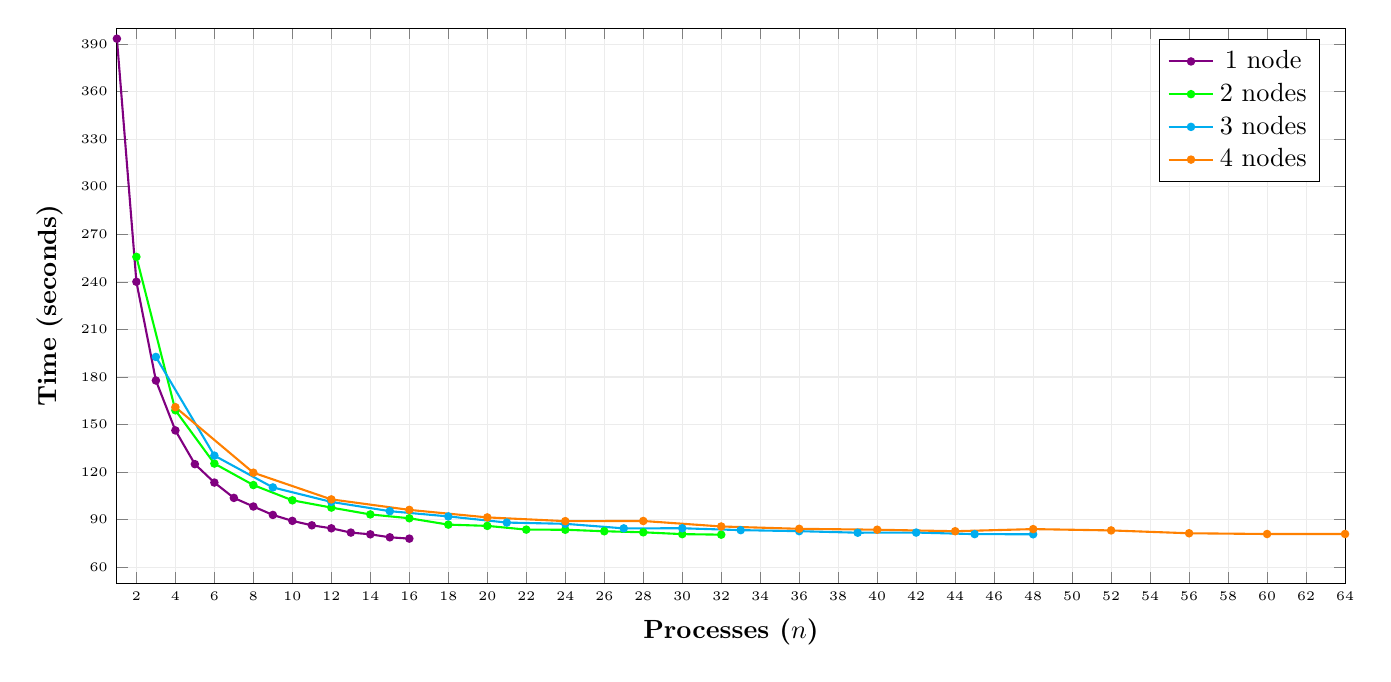
\begin{tikzpicture}[scale=0.95]
\pgfplotsset{
    tick label style = {font=\tiny}
}
\begin{axis}[
    grid=both,
    scaled y ticks = false,
    scaled x ticks = false,
   	width=18cm,
    height=9cm,
	grid style={gray!15},
    xlabel={\textbf{Processes ($n$)}},
    ylabel={\textbf{Time (seconds)}},
    xmin=1, xmax=64,
    ymin=50, ymax=400,
    xtick distance=2,
    ytick distance=30,
    xmajorgrids=true,ymajorgrids=true,
    every axis plot/.append style={thick}
]
\addplot[color=violet, mark=*, mark options={scale=0.6}]
    coordinates {
    (1,393.381)(2,240.056)(3,177.795)(4,146.297)(5,125.038)(6,113.413)(7,103.750)(8,98.319)(9,92.997)(10,89.255)(11,86.448)(12,84.564)(13,81.865)(14,80.770)(15,78.891)(16,78.059)    
    };
\addlegendentry{1 node}
\addplot[color=green, mark=*, mark options={scale=0.6}]
    coordinates {
    (2,255.793)(4,159.008)(6,125.388)(8,111.840)(10,102.222)(12,97.635)(14,93.311)(16,90.902)(18,86.881)(20,86.098)(22,83.737)(24,83.656)(26,82.708)(28,82.043)(30,80.893)(32,80.557)
    };
\addlegendentry{2 nodes}
\addplot[color=cyan, mark=*, mark options={scale=0.6}]
    coordinates {
    (3,192.649)(6,130.415)(9,110.351)(12,101.205)(15,95.371)(18,92.064)(21,88.180)(24,87.397)(27,84.521)(30,84.595)(33,83.412)(36,82.761)(39,81.784)(42,81.884)(45,80.902)(48,80.798)    
    };
\addlegendentry{3 nodes}
\addplot[color=orange, mark=*, mark options={scale=0.6}]
    coordinates {
    (4,160.965)(8,119.638)(12,102.803)(16,96.186)(20,91.436)(24,89.091)(28,89.187)(32,85.718)(36,84.241)(40,83.676)(44,82.731)(48,84.065)(52,83.229)(56,81.431)(60,80.966)(64,80.974)
    };
\addlegendentry{4 nodes}
\end{axis}
\end{tikzpicture}
\caption{Time (seconds) against MPI processes ($n$) for $n=\{1,...,64\}, p=0.01, d=20000$}
        \label{fig:ProcTime20}
\end{figure}

The trend lines observed in Figure \ref{fig:ProcTime20}, when compared with the processes-per-node view in Figure \ref{fig:ProcTimePerNode20} also show diminishing returns when more processes (and hence cores) are used per node.

\hspace{-0.5cm}\begin{minipage}[t]{0.4\textwidth}
  \centering\raisebox{\dimexpr \topskip-\height}{%
	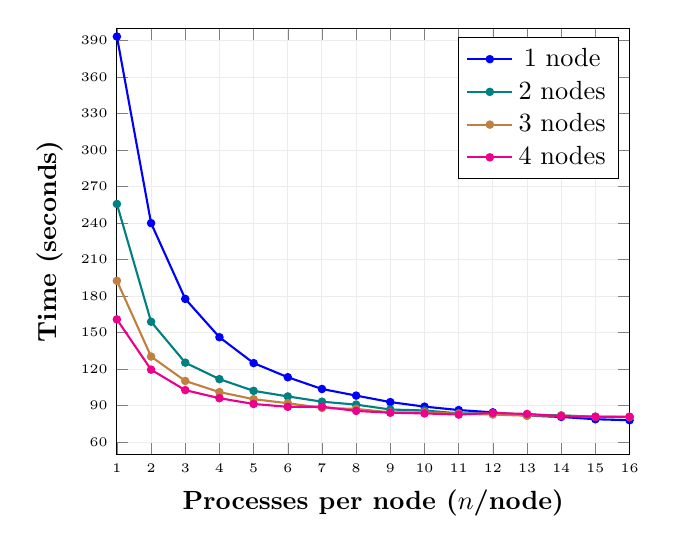
\begin{tikzpicture}[scale=0.95]
\pgfplotsset{
    tick label style = {font=\tiny}
}
\begin{axis}[
    grid=both,
    scaled y ticks = false,
    scaled x ticks = false,
	grid style={gray!15},
    xlabel={\textbf{Processes per node ($n$/node)}},
    ylabel={\textbf{Time (seconds)}},
    xmin=1, xmax=16,
    ymin=50, ymax=400,
    xtick distance=1,
    ytick distance=30,
    xmajorgrids=true,ymajorgrids=true,
    every axis plot/.append style={thick}
]
\addplot[color=blue, mark=*, mark options={scale=0.6}]
    coordinates {
    (1,393.381)(2,240.056)(3,177.795)(4,146.297)(5,125.038)(6,113.413)(7,103.750)(8,98.319)(9,92.997)(10,89.255)(11,86.448)(12,84.564)(13,81.865)(14,80.770)(15,78.891)(16,78.059)    
    };
\addlegendentry{1 node}
\addplot[color=teal, mark=*, mark options={scale=0.6}]
    coordinates {
    (1,255.793)(2,159.008)(3,125.388)(4,111.840)(5,102.222)(6,97.635)(7,93.311)(8,90.902)(9,86.881)(10,86.098)(11,83.737)(12,83.656)(13,82.708)(14,82.043)(15,80.893)(16,80.557)
    };
\addlegendentry{2 nodes}
\addplot[color=brown, mark=*, mark options={scale=0.6}]
    coordinates {
    (1,192.649)(2,130.415)(3,110.351)(4,101.205)(5,95.371)(6,92.064)(7,88.180)(8,87.397)(9,84.521)(10,84.595)(11,83.412)(12,82.761)(13,81.784)(14,81.884)(15,80.902)(16,80.798)    
    };
\addlegendentry{3 nodes}
\addplot[color=magenta, mark=*, mark options={scale=0.6}]
    coordinates {
    (1,160.965)(2,119.638)(3,102.803)(4,96.186)(5,91.436)(6,89.091)(7,89.187)(8,85.718)(9,84.241)(10,83.676)(11,82.731)(12,84.065)(13,83.229)(14,81.431)(15,80.966)(16,80.974)
    };
\addlegendentry{4 nodes}
\end{axis}
\end{tikzpicture}
}
  \captionof{figure}{Time (seconds) against MPI processes per node ($n$/node) for $n=\{1,...,64\}, p=0.01, d=20000$}
        \label{fig:ProcTimePerNode20}
\end{minipage}\hspace{1.5cm}
\begin{minipage}[t]{0.55\textwidth}
As work is divided between more processes on a single node, the time taken decreases in line with diminishing returns. Also running the relaxation across more nodes (i.e. 1 node running 1 process compared to 3 nodes running 1 process on separate dedicated nodes) significantly reduces the time required to complete the matrix relaxation as the capacity of resources on a given node (memory, network bandwidth etc.) is made available exclusively to one process with the a greater division of work. 
\\
\\
The diminishing returns trend means that for larger values of $n/node$ there is a general convergence in runtimes as all start to take similar amounts of time to complete the relaxation. Notably from $n/node=10$ upwards the messaging overhead across 4 heavily populated nodes means that it starts to become faster to run the program on just 1 node with 16 processes rather than 16 processes per node across 4 nodes.
\end{minipage}

\hspace{-0.5cm}\begin{minipage}[t]{0.4\textwidth}
  \centering\raisebox{\dimexpr \topskip-\height}{%
	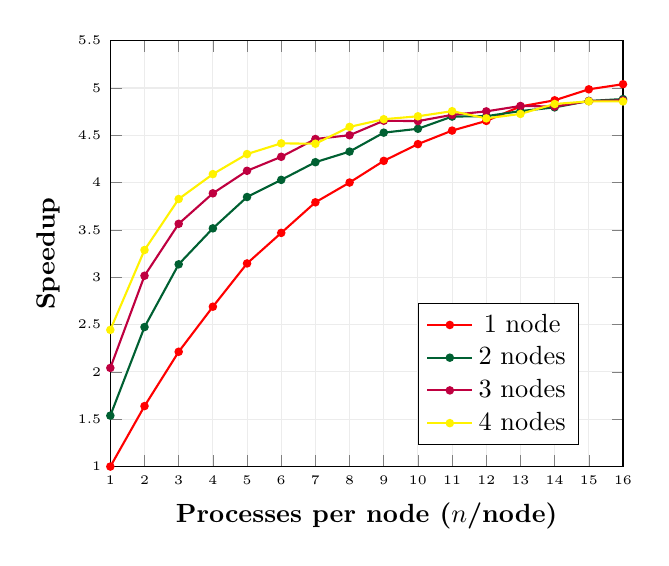
\begin{tikzpicture}[scale=0.95]
\pgfplotsset{
    tick label style = {font=\tiny}
}
\begin{axis}[
    grid=both,
    scaled y ticks = false,
    scaled x ticks = false,
	grid style={gray!15},
    xlabel={\textbf{Processes per node ($n$/node)}},
    ylabel={\textbf{Speedup}},
    xmin=1, xmax=16,
    ymin=1, ymax=5.5,
    xtick distance=1,
    ytick distance=0.5,
    legend style={at={(0.6,0.05)},anchor=south west},
    xmajorgrids=true,ymajorgrids=true,
    every axis plot/.append style={thick}
]
\addplot[color=red, mark=*, mark options={scale=0.6}]
    coordinates {
    (1,1.000)(2,1.639)(3,2.213)(4,2.689)(5,3.146)(6,3.469)(7,3.792)(8,4.001)(9,4.230)(10,4.407)(11,4.550)(12,4.652)(13,4.805)(14,4.870)(15,4.986)(16,5.040)
    };
\addlegendentry{1 node}
\addplot[color=forestgreen, mark=*, mark options={scale=0.6}]
    coordinates {
    (1,1.538)(2,2.474)(3,3.137)(4,3.517)(5,3.848)(6,4.029)(7,4.216)(8,4.328)(9,4.528)(10,4.569)(11,4.698)(12,4.702)(13,4.756)(14,4.795)(15,4.863)(16,4.883)
    };
\addlegendentry{2 nodes}
\addplot[color=purple, mark=*, mark options={scale=0.6}]
    coordinates {
    (1,2.042)(2,3.016)(3,3.565)(4,3.887)(5,4.125)(6,4.273)(7,4.461)(8,4.501)(9,4.654)(10,4.650)(11,4.716)(12,4.753)(13,4.810)(14,4.804)(15,4.862)(16,4.869)
    };
\addlegendentry{3 nodes}
\addplot[color=yellow, mark=*, mark options={scale=0.6}]
    coordinates {
    (1,2.444)(2,3.288)(3,3.827)(4,4.090)(5,4.302)(6,4.415)(7,4.411)(8,4.589)(9,4.670)(10,4.701)(11,4.755)(12,4.679)(13,4.726)(14,4.831)(15,4.859)(16,4.858)
    };
\addlegendentry{4 nodes}
\end{axis}
\end{tikzpicture}
}
  \captionof{figure}{Speedup against MPI processes per node ($n$/node) for $n=\{1,...,64\}, p=0.01, d=20000$}
        \label{fig:ProcSpeedupPerNode20}
\end{minipage}\hspace{1.5cm}
\begin{minipage}[t]{0.55\textwidth}
As seen in Figure \ref{fig:ProcSpeedupPerNode20}, the speedup was limited by the slow messaging overheads between processors, which increases when the number of processes increase. The asymptotic trend in runtime, speedup and efficiency observed is nearly identical across 1-4 nodes which seems to imply that the cost of messaging between nodes becomes less significant than memory access speeds when using a suitably large problem size (larger value of $d$).
\end{minipage}

\hspace{-0.5cm}\begin{minipage}[t]{0.4\textwidth}
  \centering\raisebox{\dimexpr \topskip-\height}{%
	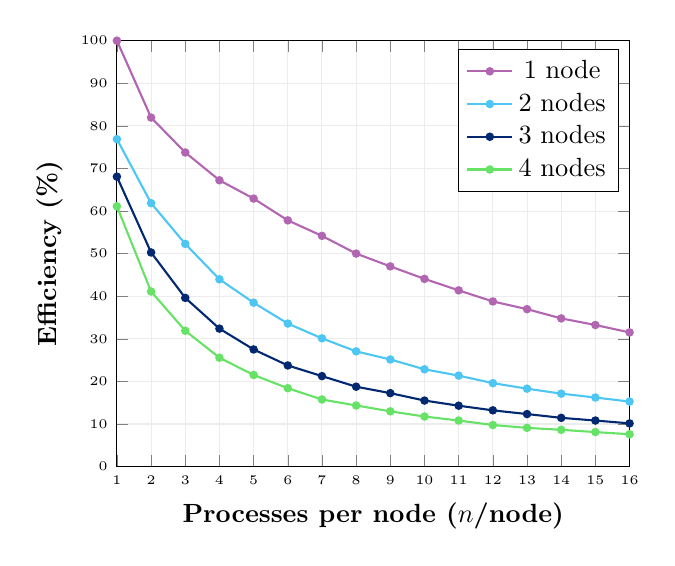
\begin{tikzpicture}[scale=0.95]
\pgfplotsset{
    tick label style = {font=\tiny}
}
\begin{axis}[
    grid=both,
    scaled y ticks = false,
    scaled x ticks = false,
	grid style={gray!15},
    xlabel={\textbf{Processes per node ($n$/node)}},
    ylabel={\textbf{Efficiency (\%)}},
    xmin=1, xmax=16,
    ymin=0, ymax=100,
    xtick distance=1,
    ytick distance=10,
    xmajorgrids=true,ymajorgrids=true,
    every axis plot/.append style={thick}
]
\addplot[color=violet!60, mark=*, mark options={scale=0.6}]
    coordinates {
    (1,100.00)(2,81.94)(3,73.75)(4,67.22)(5,62.92)(6,57.81)(7,54.17)(8,50.01)(9,47.00)(10,44.07)(11,41.37)(12,38.77)(13,36.96)(14,34.79)(15,33.24)(16,31.50)    
    };
\addlegendentry{1 node}
\addplot[color=cyan!70, mark=*, mark options={scale=0.6}]
    coordinates {
    (1,76.89)(2,61.85)(3,52.29)(4,43.97)(5,38.48)(6,33.58)(7,30.11)(8,27.05)(9,25.15)(10,22.84)(11,21.35)(12,19.59)(13,18.29)(14,17.12)(15,16.21)(16,15.26)
    };
\addlegendentry{2 nodes}
\addplot[color=darkindigo, mark=*, mark options={scale=0.6}]
    coordinates {
    (1,68.07)(2,50.27)(3,39.61)(4,32.39)(5,27.50)(6,23.74)(7,21.24)(8,18.75)(9,17.24)(10,15.50)(11,14.29)(12,13.20)(13,12.33)(14,11.44)(15,10.81)(16,10.14)
    };
\addlegendentry{3 nodes}
\addplot[color=good, mark=*, mark options={scale=0.6}]
    coordinates {
    (1,61.10)(2,41.10)(3,31.89)(4,25.56)(5,21.51)(6,18.40)(7,15.75)(8,14.34)(9,12.97)(10,11.75)(11,10.81)(12,9.75)(13,9.09)(14,8.63)(15,8.10)(16,7.59)    
    };
\addlegendentry{4 nodes}
\end{axis}
\end{tikzpicture}
}
  \captionof{figure}{Efficiency (\%) against MPI processes per node ($n$/node) for $n=\{1,...,64\}, p=0.01, d=20000$}
        \label{fig:ProcEfficPerNode20}
\end{minipage}\hspace{1.5cm}
\begin{minipage}[t]{0.55\textwidth}
In coursework 1 for a fixed problem size on a shared memory architecture, an almost-linear speedup was observed. Contrasted to this assignment where the speedup is significantly sub-linear. The trend of reduced speedup gains as more processes are used per node is also reflected in the efficiency trend shown in Figure \ref{fig:ProcEfficPerNode20}. 
\\
\\
As more processes are added per node, it becomes less efficient to run the relaxation (a pattern matched on 1-4 nodes). This is likely to be because more processes per node puts a greater demand on network bandwidth of the particular node - as in Figure \ref{fig:ProcTimePerNode20}, it is quicker to execute the relaxation when nodes are not heavily populated with running processes. For a fixed problem size the efficiency is near to an exponential decrease when extra processes are run. This again is in accordance with Amdahl's law as there is a clear limit on speedup for fixed problem sizes.
\end{minipage}

\hspace{-0.5cm}\begin{minipage}[t]{0.4\textwidth}
  \centering\raisebox{\dimexpr \topskip-\height}{%
	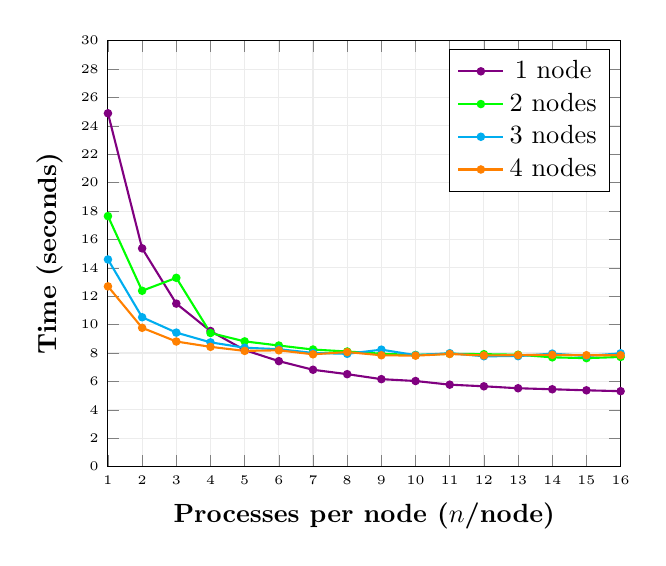
\begin{tikzpicture}[scale=0.95]
\pgfplotsset{
    tick label style = {font=\tiny}
}
\begin{axis}[
    grid=both,
    scaled y ticks = false,
    scaled x ticks = false,
	grid style={gray!15},
    xlabel={\textbf{Processes per node ($n$/node)}},
    ylabel={\textbf{Time (seconds)}},
    xmin=1, xmax=16,
    ymin=0, ymax=30,
    xtick distance=1,
    ytick distance=2,
    xmajorgrids=true,ymajorgrids=true,
    every axis plot/.append style={thick}
]
\addplot[color=violet, mark=*, mark options={scale=0.6}]
    coordinates {
    (1,24.884)(2,15.370)(3,11.478)(4,9.548)(5,8.206)(6,7.427)(7,6.818)(8,6.509)(9,6.157)(10,6.027)(11,5.769)(12,5.654)(13,5.517)(14,5.445)(15,5.371)(16,5.311)
    };
\addlegendentry{1 node}
\addplot[color=green, mark=*, mark options={scale=0.6}]
    coordinates {
    (1,17.641)(2,12.383)(3,13.294)(4,9.409)(5,8.818)(6,8.526)(7,8.244)(8,8.105)(9,7.948)(10,7.860)(11,7.948)(12,7.917)(13,7.877)(14,7.695)(15,7.637)(16,7.721)
    };
\addlegendentry{2 nodes}
\addplot[color=cyan, mark=*, mark options={scale=0.6}]
    coordinates {
    (1,14.588)(2,10.518)(3,9.436)(4,8.750)(5,8.372)(6,8.268)(7,8.006)(8,7.942)(9,8.235)(10,7.849)(11,7.982)(12,7.772)(13,7.778)(14,7.956)(15,7.785)(16,7.977)
    };
\addlegendentry{3 nodes}
\addplot[color=orange, mark=*, mark options={scale=0.6}]
    coordinates {
    (1,12.692)(2,9.776)(3,8.809)(4,8.433)(5,8.148)(6,8.189)(7,7.908)(8,8.065)(9,7.841)(10,7.813)(11,7.932)(12,7.826)(13,7.850)(14,7.871)(15,7.842)(16,7.840)
    };
\addlegendentry{4 nodes}
\end{axis}
\end{tikzpicture}
}
  \captionof{figure}{Time (seconds) against MPI processes per node ($n$/node) for $n=\{1,...,64\}, p=0.01, d=5000$}
        \label{fig:ProcTimePerNode5}
\end{minipage}\hspace{1.5cm}
\begin{minipage}[t]{0.55\textwidth}
When relaxing smaller matrices (e.g. $d=5000$) across varying sizes of $n$ it was observed that the messaging overheads caused more of an impact relative to the total runtime of the program - the same number of messages are used as in trials with larger matrix sizes, but this takes up a larger fraction of the total runtime with smaller problems. The effects of this are visible in Figures  \ref{fig:ProcTimePerNode5}, \ref{fig:ProcSpeedupPerNode5} and \ref{fig:ProcEfficPerNode5}. 
\\
\\
When smaller values of $d$ are used across varying values of $n$, it is obvious that this size of problem does not reap the rewards of having less heavily populated nodes and spreading processes across several nodes when $n/node > 5$. For example, it is much faster to keep 8 processes on one node and perform all computations there instead of spreading computations across 4 nodes (having 8 per node) despite the fact that this might divide work into more chunks. Messaging overheads are simply too large at these smaller values of $d$.
\end{minipage}

\hspace{-0.5cm}\begin{minipage}[t]{0.4\textwidth}
  \centering\raisebox{\dimexpr \topskip-\height}{%
	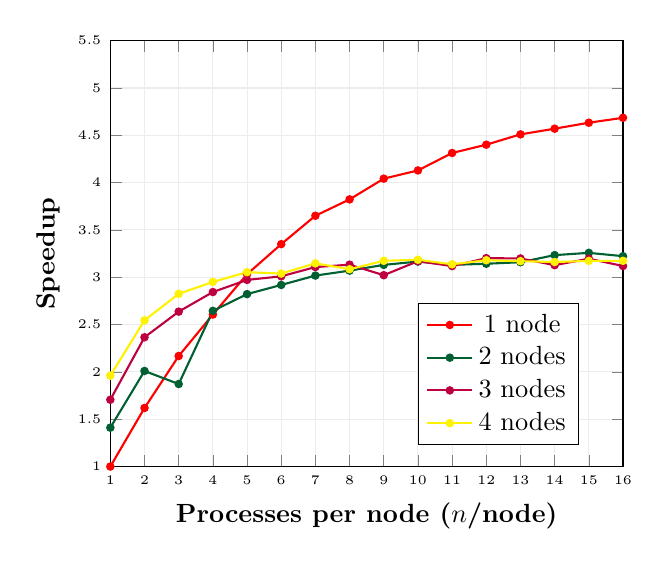
\begin{tikzpicture}[scale=0.95]
\pgfplotsset{
    tick label style = {font=\tiny}
}
\begin{axis}[
    grid=both,
    scaled y ticks = false,
    scaled x ticks = false,
	grid style={gray!15},
    xlabel={\textbf{Processes per node ($n$/node)}},
    ylabel={\textbf{Speedup}},
    xmin=1, xmax=16,
    ymin=1, ymax=5.5,
    xtick distance=1,
    ytick distance=0.5,
    legend style={at={(0.6,0.05)},anchor=south west},
    xmajorgrids=true,ymajorgrids=true,
    every axis plot/.append style={thick}
]
\addplot[color=red, mark=*, mark options={scale=0.6}]
    coordinates {
    (1,1.000)(2,1.619)(3,2.168)(4,2.606)(5,3.032)(6,3.350)(7,3.650)(8,3.823)(9,4.042)(10,4.129)(11,4.313)(12,4.401)(13,4.510)(14,4.570)(15,4.633)(16,4.685)
    };
\addlegendentry{1 node}
\addplot[color=forestgreen, mark=*, mark options={scale=0.6}]
    coordinates {
    (1,1.411)(2,2.010)(3,1.872)(4,2.645)(5,2.822)(6,2.919)(7,3.018)(8,3.070)(9,3.131)(10,3.166)(11,3.131)(12,3.143)(13,3.159)(14,3.234)(15,3.258)(16,3.223)
    };
\addlegendentry{2 nodes}
\addplot[color=purple, mark=*, mark options={scale=0.6}]
    coordinates {
    (1,1.706)(2,2.366)(3,2.637)(4,2.844)(5,2.972)(6,3.010)(7,3.108)(8,3.133)(9,3.022)(10,3.170)(11,3.118)(12,3.202)(13,3.199)(14,3.128)(15,3.196)(16,3.119)
    };
\addlegendentry{3 nodes}
\addplot[color=yellow, mark=*, mark options={scale=0.6}]
    coordinates {
    (1,1.961)(2,2.545)(3,2.825)(4,2.951)(5,3.054)(6,3.039)(7,3.147)(8,3.085)(9,3.174)(10,3.185)(11,3.137)(12,3.180)(13,3.170)(14,3.161)(15,3.173)(16,3.174)
    };
\addlegendentry{4 nodes}
\end{axis}
\end{tikzpicture}
}
  \captionof{figure}{Speedup against MPI processes per node ($n$/node) for $n=\{1,...,64\}, p=0.01, d=5000$}
        \label{fig:ProcSpeedupPerNode5}
\end{minipage}\hspace{1.5cm}
\begin{minipage}[t]{0.55\textwidth}
Contrasting Figure \ref{fig:ProcSpeedupPerNode5} with Figure \ref{fig:ProcSpeedupPerNode20}, it is clear that with a smaller problem size, the speedup values attainable by any given number of processes $n$ are smaller than with larger values of $d$, which confirms Gustafson's law. By running 4 or more processes per node it is more efficient to solve the problem for this matrix size using 1 node rather than 2 or more nodes, even though this divides the overall matrix into more chunks. The speedup attainable with 2 or more nodes is increasingly similar as the value of $n/node$ increases beyond 9. This is likely to be because at this point, nodes are becoming more heavily populated and more processes means more messages are being sent to and from the root process than there are with 1 node, which means a greater message passing overhead is incurred, limiting speedup.
\end{minipage}

\hspace{-0.5cm}\begin{minipage}[t]{0.4\textwidth}
  \centering\raisebox{\dimexpr \topskip-\height}{%
	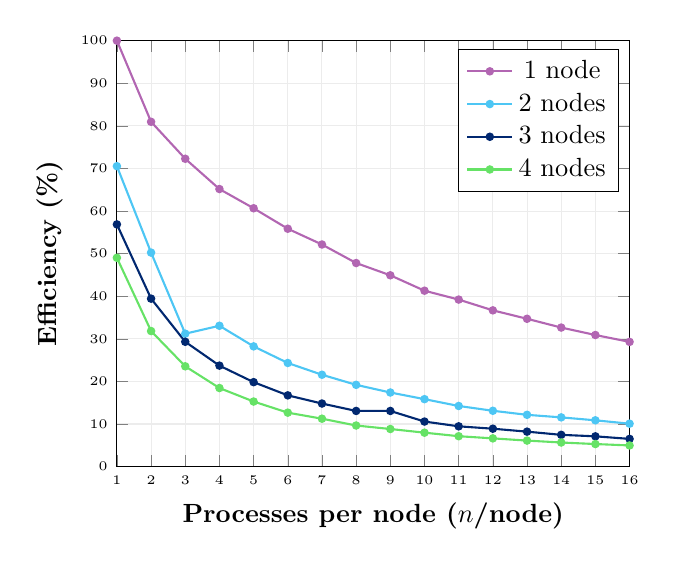
\begin{tikzpicture}[scale=0.95]
\pgfplotsset{
    tick label style = {font=\tiny}
}
\begin{axis}[
    grid=both,
    scaled y ticks = false,
    scaled x ticks = false,
	grid style={gray!15},
    xlabel={\textbf{Processes per node ($n$/node)}},
    ylabel={\textbf{Efficiency (\%)}},
    xmin=1, xmax=16,
    ymin=0, ymax=100,
    xtick distance=1,
    ytick distance=10,
    xmajorgrids=true,ymajorgrids=true,
    every axis plot/.append style={thick}
]
\addplot[color=violet!60, mark=*, mark options={scale=0.6}]
    coordinates {
    (1,100.00)(2,80.95)(3,72.27)(4,65.16)(5,60.65)(6,55.84)(7,52.14)(8,47.79)(9,44.91)(10,41.29)(11,39.21)(12,36.68)(13,34.70)(14,32.64)(15,30.89)(16,29.28)
    };
\addlegendentry{1 node}
\addplot[color=cyan!70, mark=*, mark options={scale=0.6}]
    coordinates {
    (1,70.53)(2,50.24)(3,31.20)(4,33.06)(5,28.22)(6,24.32)(7,21.56)(8,19.19)(9,17.39)(10,15.83)(11,14.23)(12,13.10)(13,12.15)(14,11.55)(15,10.86)(16,10.07)
    };
\addlegendentry{2 nodes}
\addplot[color=darkindigo, mark=*, mark options={scale=0.6}]
    coordinates {
    (1,56.86)(2,39.43)(3,29.30)(4,23.70)(5,19.82)(6,16.72)(7,14.80)(8,13.06)(9,13.06)(10,10.57)(11,9.45)(12,8.89)(13,8.20)(14,7.45)(15,7.10)(16,6.50)
    };
\addlegendentry{3 nodes}
\addplot[color=good, mark=*, mark options={scale=0.6}]
    coordinates {
    (1,49.02)(2,31.82)(3,23.54)(4,18.44)(5,15.27)(6,12.66)(7,11.24)(8,9.64)(9,8.82)(10,7.96)(11,7.13)(12,6.62)(13,6.10)(14,5.65)(15,5.29)(16,4.96)
    };
\addlegendentry{4 nodes}
\end{axis}
\end{tikzpicture}
}
  \captionof{figure}{Efficiency (\%) against MPI processes per node ($n$/node) for $n=\{1,...,64\}, p=0.01, d=5000$}
        \label{fig:ProcEfficPerNode5}
\end{minipage}\hspace{1.5cm}
\begin{minipage}[t]{0.55\textwidth}
Contrasting Figure \ref{fig:ProcEfficPerNode20} with Figure \ref{fig:ProcEfficPerNode5}, it is also clear that for a given value of $n/node$, the efficiency value will be greater if a larger matrix size (value of $d$) is used, also confirming Gustafson's law. As with $d=20000$ it is more efficient to run the program on 1 node than 2 or more for $n/node=\{1,...,16\}$. This is because in general less time is spent on communication than computation in this case so there is a more efficient use of the hardware than with 2 or more nodes in use. This difference is especially pronounced with smaller values of $d$, becoming less pronounced as the value of $d$ increases to very large scales, as this is when the fraction of execution time taken up with communication is dwarfed by the time spent doing computation.
\end{minipage}

{\color{darkpurple}
\subsubsection*{Changing the precision ($p$)}}
The next scalability experiments observed the effects of keeping a fixed matrix size and process count, whilst varying the precision value $p$ for a fixed matrix of size $d=20000$ (Figures \ref{fig:PrecTime}, \ref{fig:PrecSpeedup} and \ref{fig:PrecEffic}). These figures show the effect of increasing the problem size via reducing the precision, which causes a greater number of iterations and hence a larger total runtime. These results back up Gustafson's Law as the problem size increases so there is a reduced sequential fraction of the total runtime. When extra processors are used at suitably small values of $p$ (e.g. $p < 0.03$) it is clear that the solution can be reached in a smaller total runtime, shown by the increasing gaps between readings at each smaller value of $p$.

Comparing the general trend observed in Figure \ref{fig:PrecTime} with the shared memory coursework results, it is clear than a much smaller value of $p$ is needed in order for noticeable speedup gains to be made. With smaller values of $p$ comes more iterations which means more MPI calls are made to scatter and gather relaxed cells and reduce the logical OR operation across processes. Whilst there are benefits in parallelising the solution, there are significant messaging overheads at smaller precision values, somewhat limiting the overall speedup attainable. The value of $p$ where messaging overheads outweigh the parallelism gained is dependent on the value of $d$ and is likely to decrease as $d$ increases.

One possible side effect of the initial matrix values chosen is that a strong correlation between precision and timing is observed. As the matrices are all initialised to 1.0 on edges and 0.0 for inner values, every size of matrix will propagate values $>0$ to the centre of the matrix over each iteration. For a given precision $p$ and two matrices of sizes $d_1$ and $d_2$ where $d_1 \neq d_2$, the same number of iterations are needed for both to be relaxed with these initial values, even though the sizes are different. If the approach of random non-fixed values was used like in coursework 1, it is likely that larger values of $d$ would require more iterations making the correlation between precision and runtime less strong.
\begin{figure}[H]
\centering
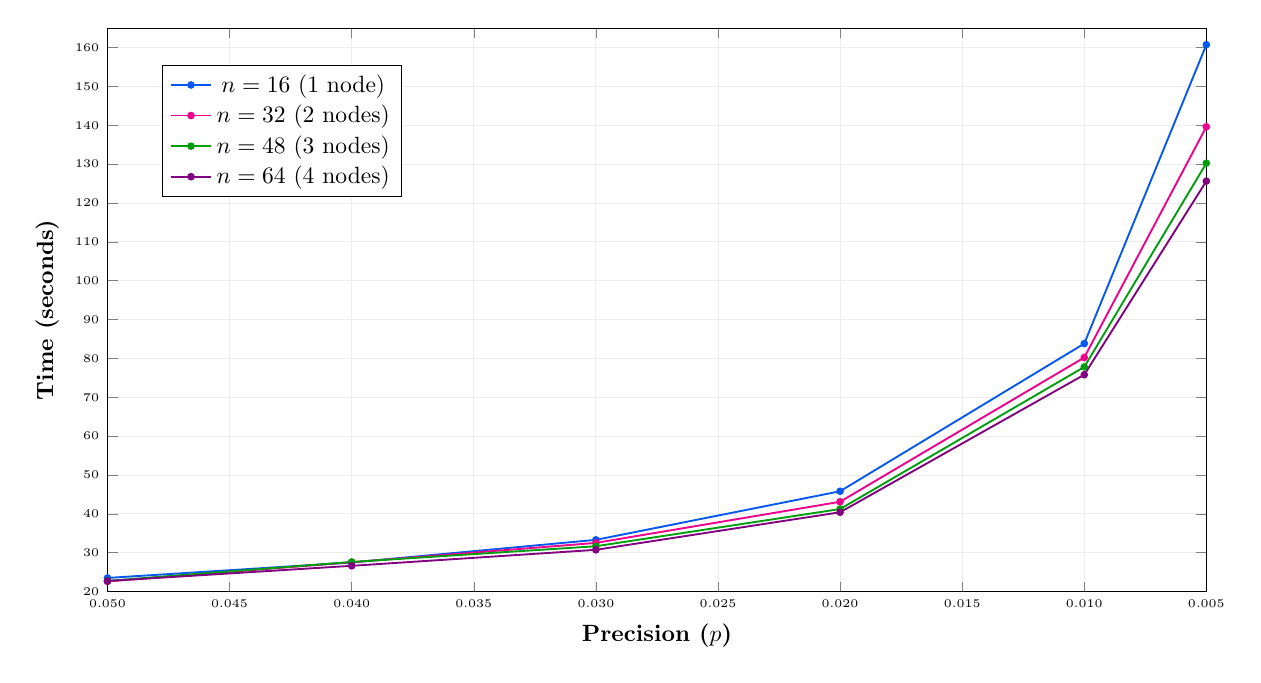
\begin{tikzpicture}[scale=0.85]
\pgfplotsset{
    tick label style = {font=\tiny}
}
\begin{axis}[
    grid=both,
    scaled y ticks = false,
    scaled x ticks = false,
   	width=18cm,
   	height=10cm,
	grid style={gray!15},
    xlabel={\textbf{Precision ($p$)}},
    ylabel={\textbf{Time (seconds)}},
    x dir=reverse,
    xmin=0.005, xmax=0.05,
    ymin=20, ymax=165,
    xtick distance=0.005,
    ytick distance=10,
    legend style={at={(0.05,0.7)},anchor=south west},
    xmajorgrids=true,ymajorgrids=true,
    every axis plot/.append style={thick},
    x tick label style={/pgf/number format/.cd,fixed,fixed zerofill,precision=3,/tikz/.cd}
]
\addplot[color=indigo, mark=*, mark options={scale=0.6}]
    coordinates {
    (0.100,15.903)(0.090,15.773)(0.080,17.746)(0.070,19.685)(0.060,18.651)(0.050,23.510)(0.040,27.490)(0.030,33.316)(0.020,45.816)(0.010,83.820)(0.005,160.744)
    };
\addlegendentry{$n=16$ (1 node)}
\addplot[color=magenta, mark=*, mark options={scale=0.6}]
    coordinates {
    (0.100,16.043)(0.090,15.884)(0.080,17.893)(0.070,19.773)(0.060,19.818)(0.050,22.636)(0.040,27.541)(0.030,32.530)(0.020,43.110)(0.010,80.234)(0.005,139.621)
    };
\addlegendentry{$n=32$ (2 nodes)}
\addplot[color=apple, mark=*, mark options={scale=0.6}]
    coordinates {
    (0.100,16.090)(0.090,15.863)(0.080,17.794)(0.070,19.793)(0.060,20.429)(0.050,22.760)(0.040,27.621)(0.030,31.671)(0.020,41.242)(0.010,77.806)(0.005,130.260)
    };
\addlegendentry{$n=48$ (3 nodes)}
\addplot[color=violet, mark=*, mark options={scale=0.6}]
    coordinates {
    (0.100,16.056)(0.090,15.875)(0.080,17.818)(0.070,19.898)(0.060,19.885)(0.050,22.717)(0.040,26.634)(0.030,30.746)(0.020,40.414)(0.010,75.811)(0.005,125.633)
    };
\addlegendentry{$n=64$ (4 nodes)}
\end{axis}
\end{tikzpicture}
\caption{Time (seconds) against Precision ($p$) for $n=\{16,32,48,64\}$, $d=20000$, $p=\{0.1,...,0.005\}$}
        \label{fig:PrecTime}
\end{figure}

From the above readings, speedup and efficiency graphs can be made (Figures \ref{fig:PrecSpeedup} and \ref{fig:PrecEffic}). 
A slight instability in results is seen at 0.003 as speedup and efficiency dips slightly. One notable difference between this test and the others is that the nodes assigned by Balena appear to be spaced further apart (in terms of node numbers alone). If the numbers do correspond to physical distance or symmetry then this could have caused the instability as messaging overheads would be greater, especially if the nodes are not sharing the same motherboard.  Figure \ref{fig:PrecSpeedup} demonstrates that regardless of the number of nodes or processes used, a smaller value of $p$ reaps larger speedups due to increased numbers of iterations and less of the total runtime being made up of sequential computation. This is in line with Gustafson's law.

From these speedup results, a graph of efficiency as $p$ varies can be constructed (Figure \ref{fig:PrecEffic}). By decreasing the value of $p$ we are increasing the overall problem size via means of increased iterations. This results in a general trend of increased efficiency. Whilst the values of efficiency for variable precision are lower on the whole compared to the shared memory assignment, this is no doubt attributable to the increase in overheads via message passing. It is clear that the problem size needs to be very large in order for this to be dwarfed by the parallelism gained.

\begin{figure}[H]
\centering
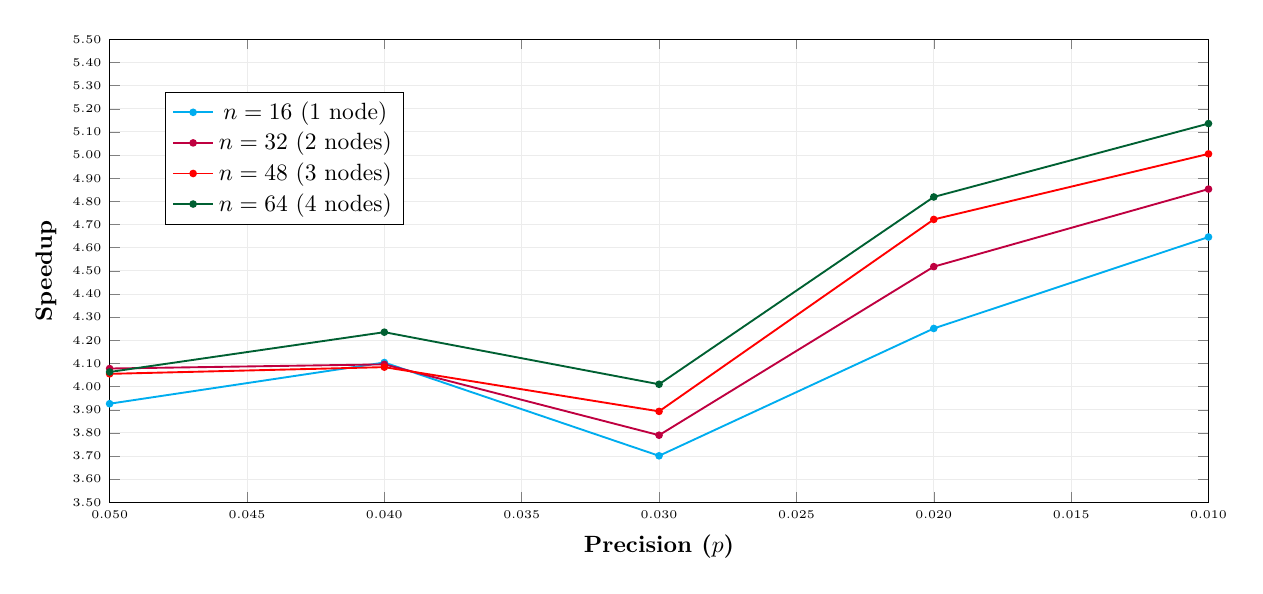
\begin{tikzpicture}[scale=0.85]
\pgfplotsset{
    tick label style = {font=\tiny}
}
\begin{axis}[
    grid=both,
    scaled y ticks = false,
    scaled x ticks = false,
   	width=18cm,
   	height=8.5cm,
	grid style={gray!15},
    xlabel={\textbf{Precision ($p$)}},
    ylabel={\textbf{Speedup}},
    x dir=reverse,
    xmin=0.01, xmax=0.05,
    ymin=3.5, ymax=5.5,
    xtick distance=0.005,
    ytick distance=0.1,
    legend style={at={(0.05,0.6)},anchor=south west},
    xmajorgrids=true,ymajorgrids=true,
    every axis plot/.append style={thick},
    y tick label style={/pgf/number format/.cd,fixed,fixed zerofill,precision=2,/tikz/.cd},
    x tick label style={/pgf/number format/.cd,fixed,fixed zerofill,precision=3,/tikz/.cd}
]
\addplot[color=cyan, mark=*, mark options={scale=0.6}]
    coordinates {
    (0.050,3.926)(0.040,4.104)(0.030,3.701)(0.020,4.251)(0.010,4.646)
    };
\addlegendentry{$n=16$ (1 node)}
\addplot[color=purple, mark=*, mark options={scale=0.6}]
    coordinates {
    (0.050,4.078)(0.040,4.096)(0.030,3.790)(0.020,4.518)(0.010,4.853)
    };
\addlegendentry{$n=32$ (2 nodes)}
\addplot[color=red, mark=*, mark options={scale=0.6}]
    coordinates {
    (0.050,4.055)(0.040,4.084)(0.030,3.893)(0.020,4.722)(0.010,5.005)
    };
\addlegendentry{$n=48$ (3 nodes)}
\addplot[color=forestgreen, mark=*, mark options={scale=0.6}]
    coordinates {
    (0.050,4.063)(0.040,4.235)(0.030,4.010)(0.020,4.819)(0.010,5.136)
    };
\addlegendentry{$n=64$ (4 nodes)}
\end{axis}
\end{tikzpicture}
\caption{Speedup against Precision ($p$) for $n=\{16,32,48,64\}$, $d=20000$, $p=\{0.1,...,0.005\}$}
        \label{fig:PrecSpeedup}
\end{figure}

\begin{figure}[H]
\centering
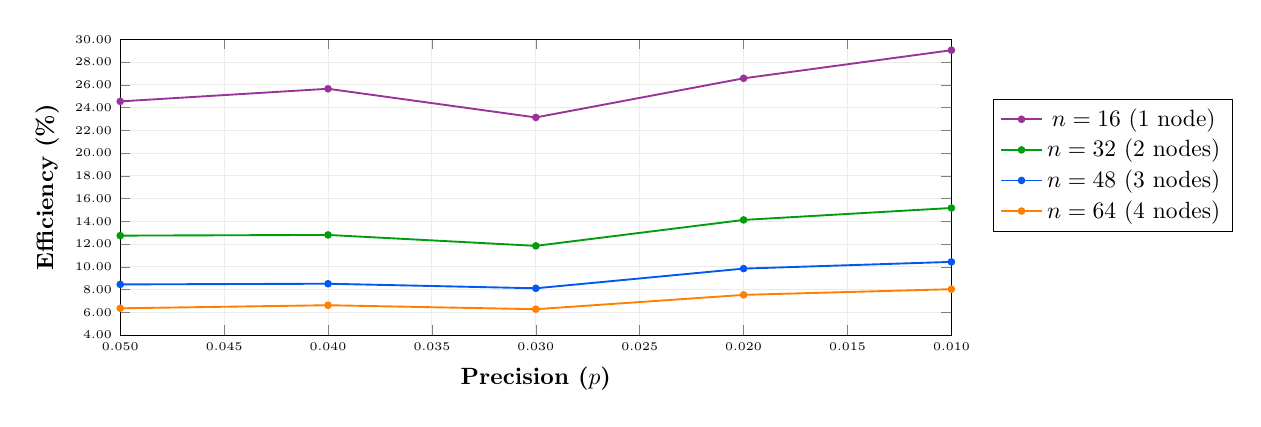
\begin{tikzpicture}[scale=0.85]
\pgfplotsset{
    tick label style = {font=\tiny}
}
\begin{axis}[
    grid=both,
    scaled y ticks = false,
    scaled x ticks = false,
   	width=14cm,
   	height=6cm,
	grid style={gray!15},
    xlabel={\textbf{Precision ($p$)}},
    ylabel={\textbf{Efficiency (\%)}},
    x dir=reverse,
    xmin=0.01, xmax=0.05,
    ymin=4, ymax=30,
    xtick distance=0.005,
    ytick distance=2,
    legend style={at={(1.05,0.35)},anchor=south west},
    xmajorgrids=true,ymajorgrids=true,
    every axis plot/.append style={thick},
    y tick label style={/pgf/number format/.cd,fixed,fixed zerofill,precision=2,/tikz/.cd},
    x tick label style={/pgf/number format/.cd,fixed,fixed zerofill,precision=3,/tikz/.cd}
]
\addplot[color=violet!80, mark=*, mark options={scale=0.6}]
    coordinates {
    (0.050,24.54)(0.040,25.65)(0.030,23.13)(0.020,26.57)(0.010,29.04)
    };
\addlegendentry{$n=16$ (1 node)}
\addplot[color=apple, mark=*, mark options={scale=0.6}]
    coordinates {
    (0.050,12.74)(0.040,12.80)(0.030,11.84)(0.020,14.12)(0.010,15.17)
    };
\addlegendentry{$n=32$ (2 nodes)}
\addplot[color=indigo, mark=*, mark options={scale=0.6}]
    coordinates {
    (0.050,8.45)(0.040,8.51)(0.030,8.11)(0.020,9.84)(0.010,10.43)
    };
\addlegendentry{$n=48$ (3 nodes)}
\addplot[color=orange, mark=*, mark options={scale=0.6}]
    coordinates {
    (0.050,6.35)(0.040,6.62)(0.030,6.27)(0.020,7.53)(0.010,8.03)
    };
\addlegendentry{$n=64$ (4 nodes)}
\end{axis}
\end{tikzpicture}
\caption{Efficiency (\%) against Precision ($p$) for $n=\{16,32,48,64\}$, $d=20000$, $p=\{0.1,...,0.005\}$}
        \label{fig:PrecEffic}
\end{figure}

As the program runs across more processes a greater number of messages are passed meaning the cost of blocking calls such as \texttt{MPI\_Scatterv} and \texttt{MPI\_Gatherv} contribute a lot to the reduced efficiency values across the spectrum of $p$ values tested compared to the shared memory assignment. It must be noted that using very small precision values (e.g. $p<0.001$) could potentially lead to a number of iterations so large that \textsl{Balena} ``times out''. Furthermore, some combinations of initial matrix values may never terminate given this value if averages never converge. See Appendix \ref{apdx:prectests} for raw data.

{\color{darkindigo}
\subsection{Varying the Matrix Dimension $d$}}
The next scalability tests involved varying the size of the matrix (size of problem) under a fixed number of processes $n$, and constant fixed precision value $p$ (Figure \ref{fig:DimTime}) to see how this affected timings. The effect of an increase in matrix dimension from $d_1$ to $d_2$ is an increase in inner cell count by $(d_2-2)^2 - (d_1-2)^2$. In other words, the matrix dimension is not linear with the number of cells to relax.

As mentioned, Gustafson's Law states that the problem size scales with the number of processors $n$ which means that speedup is not bound by $n$ if larger problem sizes are considered \cite{gustafson1988}. The raw data in Appendix \ref{apdx:dimtime} shows this too - values for speedup and efficiency increase as the matrix dimension increases to larger sizes (scales). This is consistent with the graph of dimension $d$ against time for various fixed process counts $n=\{16,32,48,64\}$ shown in Figure \ref{fig:DimTime} - larger fixed values of $n$ eventually produced reduced execution times as the matrix size scales to larger values ($>20000$), with the difference in execution times becoming more pronounced as $d$ increases beyond this value.  For smaller problem sizes ($d<20000$) the difference in execution times is far less pronounced, reinforcing the point that parallelism is only worth the initial overhead in process and data management management (e.g. work allocation, messaging overheads) if the problem is sufficiently large such that the initial parallel overheads do not dominate.

\begin{figure}[H]
\centering
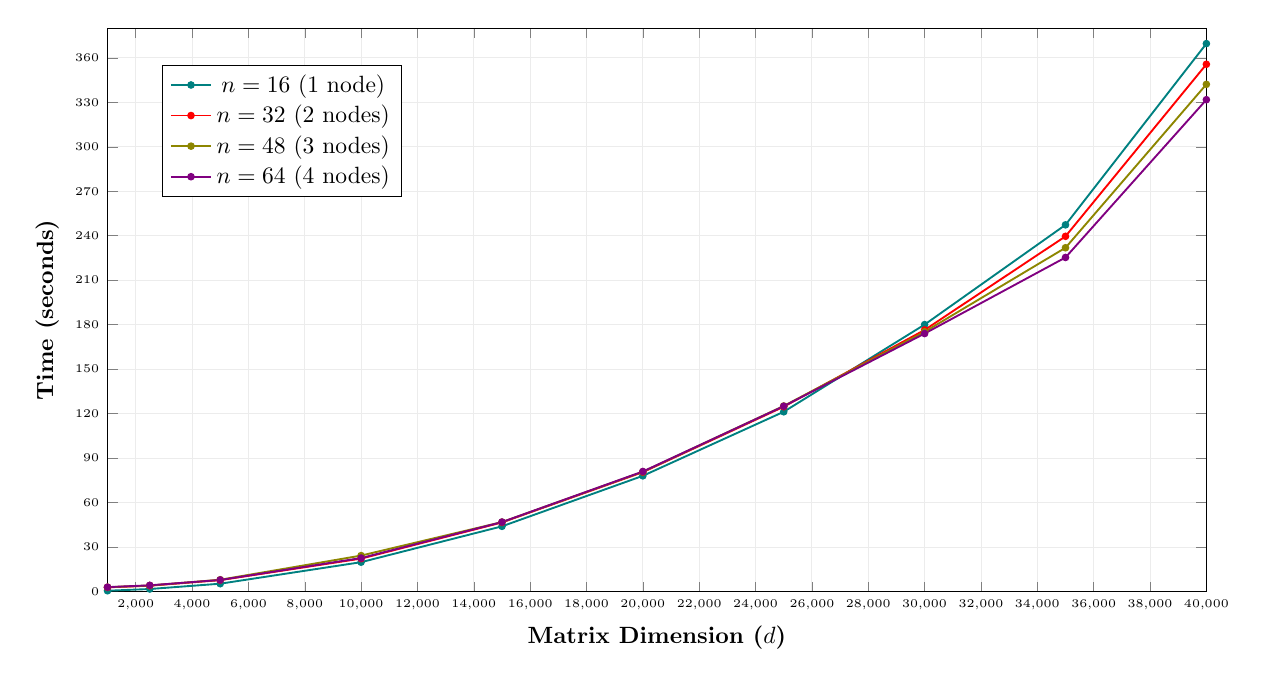
\begin{tikzpicture}[scale=0.85]
\pgfplotsset{
    tick label style = {font=\tiny}
}
\begin{axis}[
    grid=both,
    scaled y ticks = false,
    scaled x ticks = false,
   	width=18cm,
   	height=10cm,
   	legend style={at={(0.05,0.7)},anchor=south west},
	grid style={gray!15},
    xlabel={\textbf{Matrix Dimension ($d$)}},
    ylabel={\textbf{Time (seconds)}},
    xmin=1000, xmax=40000,
    ymin=0, ymax=380,
    xtick distance=2000,
    ytick distance=30,
    xmajorgrids=true,ymajorgrids=true,
    every axis plot/.append style={thick}
]
\addplot[color=teal, mark=*, mark options={scale=0.6}]
    coordinates {
    (1000,0.558)(2500,1.729)(5000,5.311)(10000,19.827)(15000,44.003)(20000,78.059)(25000,121.269)(30000,180.069)(35000,247.335)(40000,369.563)       
    };
\addlegendentry{$n=16$ (1 node)}
\addplot[color=red, mark=*, mark options={scale=0.6}]
    coordinates {
   (1000,2.857)(2500,3.976)(5000,7.721)(10000,22.240)(15000,46.634)(20000,80.557)(25000,124.689)(30000,176.438)(35000,239.596)(40000,355.627)
  	};
\addlegendentry{$n=32$ (2 nodes)}
\addplot[color=olive, mark=*, mark options={scale=0.6}]
    coordinates {
    (1000,2.922)(2500,4.067)(5000,7.977)(10000,24.278)(15000,46.859)(20000,80.798)(25000,125.163)(30000,175.184)(35000,231.884)(40000,342.105)   
    };
\addlegendentry{$n=48$ (3 nodes)}
\addplot[color=violet, mark=*, mark options={scale=0.6}]
    coordinates {
    (1000,2.992)(2500,4.221)(5000,7.840)(10000,22.610)(15000,46.872)(20000,80.974)(25000,125.031)(30000,174.020)(35000,225.337)(40000,331.733)
    };
\addlegendentry{$n=64$ (4 nodes)}
\end{axis}
\end{tikzpicture}
\caption{Time (seconds) against Matrix Dimension ($d$) for $d=\{1000,...,40000\}, p=0.01, n=\{16,32,48,64\}$}
        \label{fig:DimTime}
\end{figure}

Figures \ref{fig:DimSpeedup} and \ref{fig:DimEffic} show the overall trend in speedup and efficiency for a variety of matrix sizes - at values of $d$ beyond 25000 the program using 1 process on 1 node will timeout on Balena, meaning speedup and efficiency values cannot be calculated as there is no ``sequential'' time in order to reference against.

It is visible that for small matrix sizes ($d<10000$), greater speedup is possible using 16 processes on 1 node than 2 or more nodes all running 16 processes. This is likely to be because messaging overheads at these sizes dominate the overall execution time. As the matrix size increases, speedups using larger number of processes and nodes increases to match the same sort of values attainable by 1 node as messaging overheads eventually become dwarfed by the parallelism gained.  This pattern is reflected in Figure \ref{fig:DimEffic} - it is more efficient use of hardware when 1 node is used than 2 or more for smaller matrix sizes due to messaging overheads. There is also clearly a gain in efficiency when a given number of processes are tasked with relaxing larger matrices, which complies with Gustafson's law. 

\begin{figure}[H]
\centering
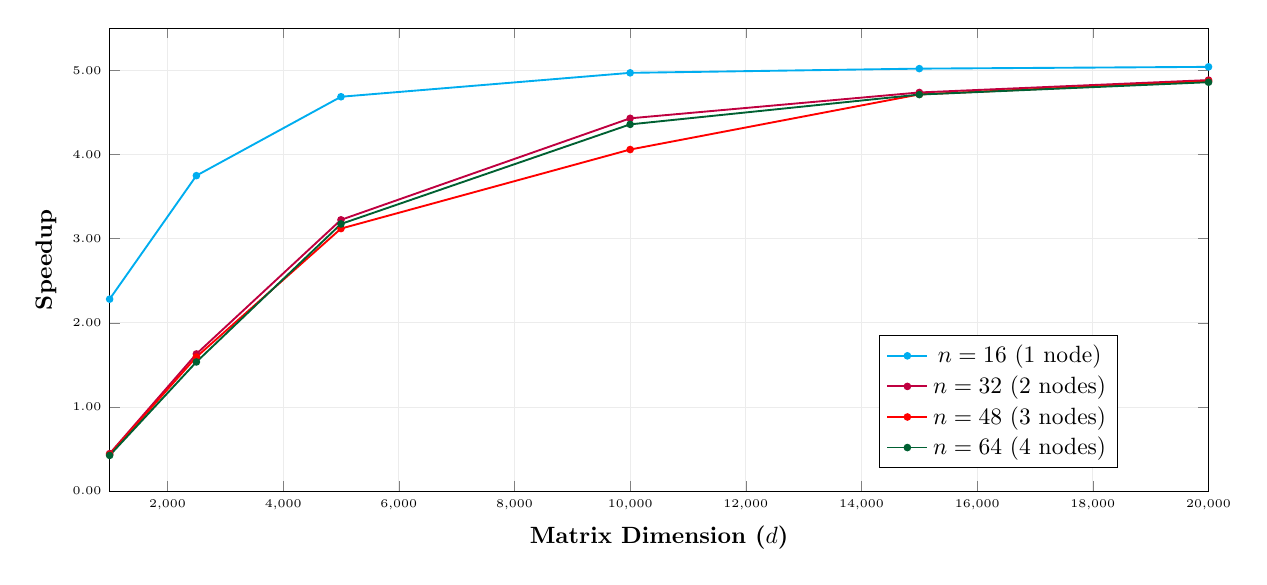
\begin{tikzpicture}[scale=0.85]
\pgfplotsset{
    tick label style = {font=\tiny}
}
\begin{axis}[
    grid=both,
    scaled y ticks = false,
    scaled x ticks = false,
   	width=18cm,
   	height=8.5cm,
	grid style={gray!15},
    xlabel={\textbf{Matrix Dimension ($d$)}},
    ylabel={\textbf{Speedup}},
    xmin=1000, xmax=20000,
    ymin=0, ymax=5.5,
    xtick distance=2000,
    ytick distance=1,
    legend style={at={(0.7,0.05)},anchor=south west},
    xmajorgrids=true,ymajorgrids=true,
    every axis plot/.append style={thick},
    y tick label style={/pgf/number format/.cd,fixed,fixed zerofill,precision=2,/tikz/.cd},
]
\addplot[color=cyan, mark=*, mark options={scale=0.6}]
    coordinates {
    (1000,2.281)(2500,3.748)(5000,4.685)(10000,4.969)(15000,5.019)(20000,5.040)(25000,5.081)   
    };
\addlegendentry{$n=16$ (1 node)}
\addplot[color=purple, mark=*, mark options={scale=0.6}]
    coordinates {
    (1000,0.446)(2500,1.630)(5000,3.223)(10000,4.429)(15000,4.736)(20000,4.883)(25000,4.942)
    };
\addlegendentry{$n=32$ (2 nodes)}
\addplot[color=red, mark=*, mark options={scale=0.6}]
    coordinates {
    (1000,0.436)(2500,1.594)(5000,3.119)(10000,4.058)(15000,4.713)(20000,4.869)(25000,4.923)
    };
\addlegendentry{$n=48$ (3 nodes)}
\addplot[color=forestgreen, mark=*, mark options={scale=0.6}]
    coordinates {
    (1000,0.425)(2500,1.535)(5000,3.174)(10000,4.357)(15000,4.711)(20000,4.858)(25000,4.928)
    };
\addlegendentry{$n=64$ (4 nodes)}
\end{axis}
\end{tikzpicture}
\caption{Speedup against Matrix Dimension ($d$) for $d=\{1000,...,25000\}, p=0.01, n=\{16,32,48,64\}$}
        \label{fig:DimSpeedup}
\end{figure}

\begin{figure}[H]
\centering
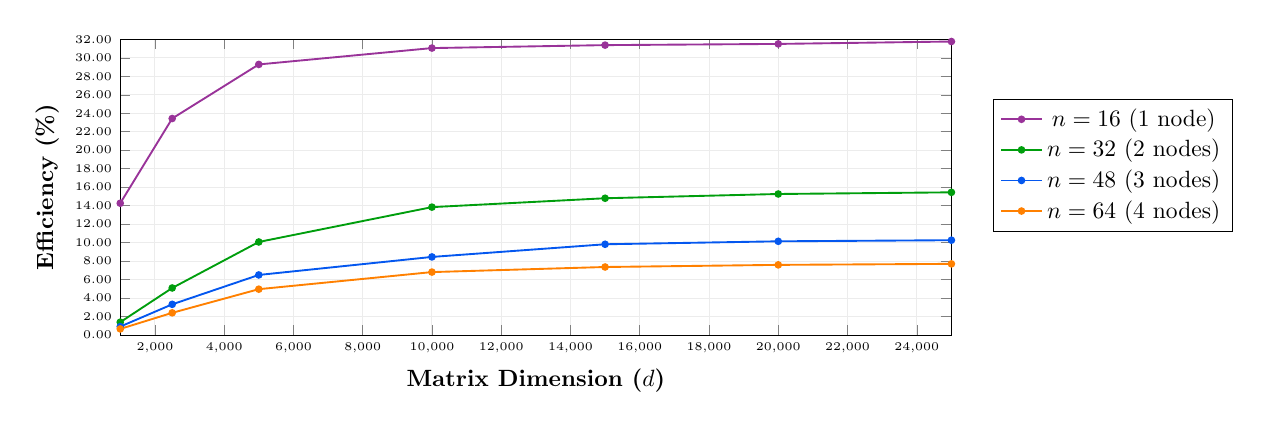
\begin{tikzpicture}[scale=0.85]
\pgfplotsset{
    tick label style = {font=\tiny}
}
\begin{axis}[
    grid=both,
    scaled y ticks = false,
    scaled x ticks = false,
   	width=14cm,
   	height=6cm,
	grid style={gray!15},
    xlabel={\textbf{Matrix Dimension ($d$)}},
    ylabel={\textbf{Efficiency (\%)}},
    xmin=1000, xmax=25000,
    ymin=0, ymax=32,
    xtick distance=2000,
    ytick distance=2,
    legend style={at={(1.05,0.35)},anchor=south west},
    xmajorgrids=true,ymajorgrids=true,
    every axis plot/.append style={thick},
    y tick label style={/pgf/number format/.cd,fixed,fixed zerofill,precision=2,/tikz/.cd},
]
\addplot[color=violet!80, mark=*, mark options={scale=0.6}]
    coordinates {
    (1000,14.26)(2500,23.43)(5000,29.28)(10000,31.05)(15000,31.37)(20000,31.50)(25000,31.76)
    };
\addlegendentry{$n=16$ (1 node)}
\addplot[color=apple, mark=*, mark options={scale=0.6}]
    coordinates {
    (1000,1.39)(2500,5.09)(5000,10.07)(10000,13.84)(15000,14.80)(20000,15.26)(25000,15.44)
    };
\addlegendentry{$n=32$ (2 nodes)}
\addplot[color=indigo, mark=*, mark options={scale=0.6}]
    coordinates {
    (1000,0.91)(2500,3.32)(5000,6.50)(10000,8.45)(15000,9.82)(20000,10.14)(25000,10.26)
    };
\addlegendentry{$n=48$ (3 nodes)}
\addplot[color=orange, mark=*, mark options={scale=0.6}]
    coordinates {
    (1000,0.66)(2500,2.40)(5000,4.96)(10000,6.81)(15000,7.36)(20000,7.59)(25000,7.70)
    };
\addlegendentry{$n=64$ (4 nodes)}
\end{axis}
\end{tikzpicture}
\caption{Efficiency (\%) against Matrix Dimension ($d$) for $d=\{1000,...,25000\}, p=0.01, n=\{16,32,48,64\}$}
        \label{fig:DimEffic}
\end{figure}

{\color{darkindigo}
\subsection{Further Speedup and Efficiency Calculations}
\label{sec:speedupeffic}}
The final scalability tests involved varying either the size of the matrix or the process count $n$ whilst the other variable was fixed, with a constant fixed precision value $p$ to see how this affected speedup (Table \ref{tbl:Speedup}) and efficiency (Table \ref{tbl:Efficiency}) measurements. The below table cells have been coloured to indicate a particularly {\color{bad}{\textbf{low}}} or {\color{good!70!black}{\textbf{high}}} value of speedup or efficiency respectively, to make it easier to see the trend in how both values vary across varying matrix dimensions and process counts. \textbf{Values have been calculated using the raw data in Appendix \ref{apdx:timespeedupefficgrids}.}

The speedup value using $n$ processors, $S_{n}$, is calculated as: $\dfrac{T_{s}+T_{p}}{T_{s}+\frac{T_{p}}{n}}$ where $T_{s}$ and $T_{p}$ account for the sequential and parallel execution times respectively \cite{gustafson1988}. The efficiency value using $n$ processors, $E_{n}$, is calculated as $\frac{S_{n}}{n}$. It is clear from these experiments that the value of $n$ which produces the largest $E_{n}$ (i.e. $n=1$) is not the same value of $n$ which produces the maximum $S_{n}$. A careful consideration is needed by system designers depending on whether efficient use of hardware or reduced execution time is a priority.  The rationale behind the equal division of the matrix between processes and minimising of messaging overheads was to parallelise the problem as efficiently as possible. It is clear that this efficiency is only shown in sufficiently large problem sizes.  Matrix dimensions of $d<2500$ don't show much benefit from this effort. 

In fact, for $d\leq1000$ on 2 or more nodes, $S_{n}<1$ which means the increase in overheads by increasing $n$ to run across more than 1 node has actually made it quicker to solve this size of problem sequentially at precision $0.01$. For a fixed problem size there is indeed a natural limit on speedup, confirming Amdahl's Law. It is only once the dimension $d$ increases beyond $10000\times10000$ that the benefits of parallelism are observed in the form of larger speedups whilst more processes are executed in parallel across $n$ cores (1 process per core), confirming Gustafson's Law. For example, the greatest value of total speedup observed was 5.081 using 16 processes on 1 node with a a $25000\times25000$ matrix where the problem size is very large - $\sim \frac{(25000-2)}{16}$ rows are given to each process to relax.

There is also a general trend that efficiency is increased when larger matrices are relaxed. This is because a greater fraction of the time can be spent on computation relative to communication. It is no surprise that for a given number of processes $n$, the value of $d$ producing the most efficient computations came when $d=25000$.

Compared to the shared memory assignment, overall speedup values for a given matrix size was significantly less (e.g. the greatest value of total speedup observed in the previous assignment was 10.247 using 15 threads on a $15000\times15000$ matrix). Compared to the largest speedup of 5.081 using 16 processes on 1 node with a a $25000\times25000$ matrix, it is clear that problems are only suited to being solved in parallel on distributed memory architectures if the size of problem is suitably larger. Here, the costs of message passing are countered by the increased parallelism.

\color{black}
	\pgfplotstableset{
    color cells/.style={
        col sep=comma,
        font=\fontsize{6}{7.2}\selectfont,
        string type,
        trim cells=true,
        postproc cell content/.code={%
                \pgfkeysalso{@cell content=\rule{0cm}{0.4ex}\cellcolor{white!##1}\pgfmathtruncatemacro\number{##1}
                \ifnum\number>-1
                	\cellcolor{bad!50}
               \fi
                \ifnum\number>1
                	\cellcolor{badtoavg!50}
               \fi
               \ifnum\number>2
                	\cellcolor{avg}
               \fi
               \ifnum\number>3
                	\cellcolor{avgtogood}
               \fi
               \ifnum\number>4
               		\cellcolor{good}
               	\fi##1}%
                },
        columns/x/.style={
            column name={},
            fixed,
            postproc cell content/.code={}
        }
    }
}
\begin{table}[H]
\caption{Speedup across range of process counts ($n=\{1,...,64\}$) and matrix dimensions ($d=\{1000,...,25000\}$), with $p=0.01$.}\label{tbl:Speedup}
\centering
\pgfplotstabletypeset[color cells]{
x,1000,2500,5000,10000,15000,20000,25000
1 (1 node),1.000,1.000,1.000,1.000,1.000,1.000,1.000
2 (1 node),1.426,1.574,1.619,1.630,1.631,1.639,1.634
3 (1 node),1.638,2.059,2.168,2.189,2.194,2.213,2.215
4 (1 node),1.878,2.415,2.606,2.667,2.675,2.689,2.704
5 (1 node),2.034,2.819,3.032,3.110,3.121,3.146,3.145
6 (1 node),2.094,3.064,3.350,3.425,3.464,3.469,3.484
7 (1 node),2.122,3.252,3.650,3.748,3.756,3.792,3.835
8 (1 node),2.249,3.376,3.823,3.951,3.968,4.001,4.012
9 (1 node),2.269,3.466,4.042,4.155,4.200,4.230,4.234
10 (1 node),2.269,3.509,4.129,4.325,4.342,4.407,4.381
11 (1 node),2.310,3.599,4.313,4.492,4.522,4.550,4.559
12 (1 node),1.980,3.579,4.401,4.582,4.630,4.652,4.671
13 (1 node),2.290,3.595,4.510,4.737,4.758,4.805,4.814
14 (1 node),2.277,3.583,4.570,4.799,4.843,4.870,4.899
15 (1 node),1.711,3.710,4.633,4.924,4.976,4.986,5.023
16 (1 node),2.281,3.748,4.685,4.969,5.019,5.040,5.081
2 (2 nodes),0.416,1.189,1.411,1.508,1.524,1.538,1.199
4 (2 nodes),0.431,1.312,2.010,2.360,2.434,2.474,2.490
6 (2 nodes),0.461,1.435,1.872,2.962,3.079,3.137,3.176
8 (2 nodes),0.461,1.530,2.645,3.284,3.440,3.517,3.550
10 (2 nodes),0.465,1.580,2.822,3.564,3.737,3.848,3.885
12 (2 nodes),0.447,1.598,2.919,3.732,3.919,4.029,4.077
14 (2 nodes),0.461,1.538,3.018,3.893,4.108,4.216,4.276
16 (2 nodes),0.460,1.628,3.070,3.669,4.211,4.328,4.393
18 (2 nodes),0.455,1.588,3.131,4.106,4.336,4.528,4.517
20 (2 nodes),0.449,1.626,3.166,4.167,4.407,4.569,4.603
22 (2 nodes),0.426,1.632,3.131,4.261,4.513,4.698,4.694
24 (2 nodes),0.459,1.621,3.143,4.298,4.558,4.702,4.763
26 (2 nodes),0.454,1.622,3.159,4.359,4.623,4.756,4.828
28 (2 nodes),0.455,1.627,3.234,4.371,4.654,4.795,4.872
30 (2 nodes),0.449,1.637,3.258,4.425,4.691,4.863,4.921
32 (2 nodes),0.446,1.630,3.223,4.429,4.736,4.883,4.942
3 (3 nodes),0.436,1.185,1.706,1.953,2.006,2.042,2.045
6 (3 nodes),0.457,1.442,2.366,2.838,2.961,3.016,3.055
9 (3 nodes),0.461,1.526,2.637,3.325,3.476,3.565,3.601
12 (3 nodes),0.454,1.585,2.844,3.585,3.777,3.887,3.927
15 (3 nodes),0.465,1.596,2.972,3.823,4.024,4.125,4.107
18 (3 nodes),0.462,1.607,3.010,3.943,4.165,4.273,4.326
21 (3 nodes),0.452,1.625,3.108,4.052,4.293,4.461,4.467
24 (3 nodes),0.451,1.601,3.133,4.121,4.367,4.501,4.560
27 (3 nodes),0.455,1.648,3.022,4.205,4.468,4.654,4.649
30 (3 nodes),0.451,1.635,3.170,4.254,4.529,4.650,4.708
33 (3 nodes),0.446,1.630,3.118,4.295,4.580,4.716,4.710
36 (3 nodes),0.447,1.633,3.202,4.320,4.601,4.753,4.810
39 (3 nodes),0.444,1.598,3.199,4.372,4.653,4.810,4.814
42 (3 nodes),0.348,1.532,3.128,4.382,4.681,4.804,4.861
45 (3 nodes),0.423,1.577,3.196,4.057,4.710,4.862,4.919
48 (3 nodes),0.436,1.594,3.119,4.058,4.713,4.869,4.923
4 (4 nodes),0.418,1.303,1.961,2.316,2.387,2.444,2.433
8 (4 nodes),0.460,1.507,2.545,3.139,3.268,3.288,3.367
12 (4 nodes),0.458,1.576,2.825,3.564,3.727,3.827,3.862
16 (4 nodes),0.459,1.612,2.951,3.533,3.975,4.090,4.084
20 (4 nodes),0.462,1.624,3.054,3.621,4.170,4.302,4.290
24 (4 nodes),0.443,1.603,3.039,4.044,4.281,4.415,4.458
28 (4 nodes),0.455,1.609,3.147,4.153,4.393,4.411,4.573
32 (4 nodes),0.446,1.631,3.085,4.185,4.434,4.589,4.641
36 (4 nodes),0.453,1.627,3.174,4.260,4.341,4.670,4.714
40 (4 nodes),0.440,1.626,3.185,4.263,4.548,4.701,4.694
44 (4 nodes),0.444,1.600,3.137,4.324,4.600,4.755,4.739
48 (4 nodes),0.431,1.570,3.180,4.329,4.614,4.679,4.767
52 (4 nodes),0.421,1.612,3.170,4.370,4.651,4.726,4.805
56 (4 nodes),0.407,1.553,3.161,4.361,4.694,4.831,4.889
60 (4 nodes),0.428,1.553,3.173,4.393,4.692,4.859,4.915
64 (4 nodes),0.425,1.535,3.174,4.357,4.711,4.858,4.928
}
\end{table}

\color{black}
	\pgfplotstableset{
    color cells/.style={
        col sep=comma,
        font=\fontsize{6}{7.2}\selectfont,
        string type,
        trim cells=true,
        postproc cell content/.code={%
                \pgfkeysalso{@cell content=\rule{0cm}{0.4ex}\cellcolor{white!##1}\pgfmathtruncatemacro\number{##1}
                \ifnum\number>-1
                	\cellcolor{bad!50}
               \fi
                \ifnum\number>5
                	\cellcolor{badtoavg!50}
               \fi
               \ifnum\number>15
                	\cellcolor{avg}
               \fi
               \ifnum\number>50
                	\cellcolor{avgtogood}
               \fi
               \ifnum\number>70
               		\cellcolor{good}
               	\fi##1}%
                },
        columns/x/.style={
            column name={},
            fixed,
            postproc cell content/.code={}
        }
    }
}
\begin{table}[H]
\caption{Efficiency across range of process counts ($n=\{1,...,64\}$) and matrix dimensions ($d=\{1000,...,25000\}$), with $p=0.01$.}\label{tbl:Efficiency}
\centering
\pgfplotstabletypeset[color cells]{
x,1000,2500,5000,10000,15000,20000,25000
1 (1 node),100.00,100.00,100.00,100.00,100.00,100.00,100.00
2 (1 node),71.28,78.69,80.95,81.48,81.56,81.94,81.69
3 (1 node),54.61,68.63,72.27,72.98,73.14,73.75,73.82
4 (1 node),46.94,60.37,65.16,66.68,66.87,67.22,67.59
5 (1 node),40.67,56.38,60.65,62.20,62.41,62.92,62.91
6 (1 node),34.90,51.07,55.84,57.08,57.74,57.81,58.07
7 (1 node),30.31,46.46,52.14,53.54,53.66,54.17,54.78
8 (1 node),28.11,42.19,47.79,49.39,49.60,50.01,50.16
9 (1 node),25.21,38.51,44.91,46.17,46.67,47.00,47.04
10 (1 node),22.69,35.09,41.29,43.25,43.42,44.07,43.81
11 (1 node),21.00,32.71,39.21,40.84,41.11,41.37,41.45
12 (1 node),16.50,29.82,36.68,38.18,38.58,38.77,38.93
13 (1 node),17.61,27.65,34.70,36.44,36.60,36.96,37.03
14 (1 node),16.27,25.59,32.64,34.28,34.60,34.79,34.99
15 (1 node),11.41,24.73,30.89,32.83,33.17,33.24,33.49
16 (1 node),14.26,23.43,29.28,31.05,31.37,31.50,31.76
2 (2 nodes),20.82,59.45,70.53,75.39,76.18,76.89,59.93
4 (2 nodes),10.78,32.81,50.24,58.99,60.85,61.85,62.26
6 (2 nodes),7.68,23.92,31.20,49.36,51.32,52.29,52.93
8 (2 nodes),5.76,19.12,33.06,41.04,43.00,43.97,44.38
10 (2 nodes),4.65,15.80,28.22,35.64,37.37,38.48,38.85
12 (2 nodes),3.73,13.32,24.32,31.10,32.66,33.58,33.97
14 (2 nodes),3.29,10.99,21.56,27.81,29.34,30.11,30.54
16 (2 nodes),2.87,10.18,19.19,22.93,26.32,27.05,27.45
18 (2 nodes),2.53,8.82,17.39,22.81,24.09,25.15,25.09
20 (2 nodes),2.24,8.13,15.83,20.83,22.04,22.84,23.02
22 (2 nodes),1.94,7.42,14.23,19.37,20.51,21.35,21.34
24 (2 nodes),1.91,6.75,13.10,17.91,18.99,19.59,19.85
26 (2 nodes),1.75,6.24,12.15,16.76,17.78,18.29,18.57
28 (2 nodes),1.63,5.81,11.55,15.61,16.62,17.12,17.40
30 (2 nodes),1.50,5.46,10.86,14.75,15.64,16.21,16.40
32 (2 nodes),1.39,5.09,10.07,13.84,14.80,15.26,15.44
3 (3 nodes),14.54,39.50,56.86,65.11,66.85,68.07,68.18
6 (3 nodes),7.62,24.03,39.43,47.30,49.35,50.27,50.91
9 (3 nodes),5.12,16.96,29.30,36.94,38.63,39.61,40.01
12 (3 nodes),3.78,13.21,23.70,29.88,31.47,32.39,32.72
15 (3 nodes),3.10,10.64,19.82,25.48,26.83,27.50,27.38
18 (3 nodes),2.57,8.93,16.72,21.91,23.14,23.74,24.03
21 (3 nodes),2.15,7.74,14.80,19.30,20.44,21.24,21.27
24 (3 nodes),1.88,6.67,13.06,17.17,18.20,18.75,19.00
27 (3 nodes),1.69,6.10,11.19,15.58,16.55,17.24,17.22
30 (3 nodes),1.50,5.45,10.57,14.18,15.10,15.50,15.69
33 (3 nodes),1.35,4.94,9.45,13.02,13.88,14.29,14.27
36 (3 nodes),1.24,4.54,8.89,12.00,12.78,13.20,13.36
39 (3 nodes),1.14,4.10,8.20,11.21,11.93,12.33,12.34
42 (3 nodes),0.83,3.65,7.45,10.43,11.15,11.44,11.57
45 (3 nodes),0.94,3.50,7.10,9.02,10.47,10.81,10.93
48 (3 nodes),0.91,3.32,6.50,8.45,9.82,10.14,10.26
4 (4 nodes),10.44,32.57,49.02,57.90,59.67,61.10,60.81
8 (4 nodes),5.74,18.84,31.82,39.24,40.85,41.10,42.09
12 (4 nodes),3.81,13.13,23.54,29.70,31.06,31.89,32.18
16 (4 nodes),2.87,10.07,18.44,22.08,24.84,25.56,25.53
20 (4 nodes),2.31,8.12,15.27,18.11,20.85,21.51,21.45
24 (4 nodes),1.85,6.68,12.66,16.85,17.84,18.40,18.58
28 (4 nodes),1.62,5.74,11.24,14.83,15.69,15.75,16.33
32 (4 nodes),1.39,5.10,9.64,13.08,13.86,14.34,14.50
36 (4 nodes),1.26,4.52,8.82,11.83,12.06,12.97,13.09
40 (4 nodes),1.10,4.07,7.96,10.66,11.37,11.75,11.74
44 (4 nodes),1.01,3.64,7.13,9.83,10.45,10.81,10.77
48 (4 nodes),0.90,3.27,6.62,9.02,9.61,9.75,9.93
52 (4 nodes),0.81,3.10,6.10,8.40,8.94,9.09,9.24
56 (4 nodes),0.73,2.77,5.65,7.79,8.38,8.63,8.73
60 (4 nodes),0.71,2.59,5.29,7.32,7.82,8.10,8.19
64 (4 nodes),0.66,2.40,4.96,6.81,7.36,7.59,7.70
}
\end{table}

\footnotesize
\bibliography{Bibliography}
\normalsize
\begin{appendices}
{\color{indigo}
\section{Compiling and Running the \texttt{distributedrelax.c} program}
\label{apdx:runprog}}
Compiling the source code can be done with \texttt{mpicc} (recommended). Once compiled into a binary file \texttt{distributedrelax}, the program is executable with customisable CLI parameters. Arguments are parsed with the getopt library\footnote{\url{https://www.gnu.org/software/libc/manual/html node/Getopt.html}}. An example compilation and run of the program might look like:	
\begin{lstlisting}[style=BashInputStyle]
    $		mpicc -Wall -std=gnu99 distributedrelax.c -o distributedrelax
    $		mpirun -np 4 ./distributedrelax -d 1000 -p 0.5 -i
\end{lstlisting}

The above runs the program using a $1000 \times 1000$ matrix with a precision of $0.5$, with info mode enabled using 4 processes.

\begin{table}[h]
\begin{center}
\caption{Program command line arguments.}
\label{tbl:CLIargs}
\begin{tabular}{|c|c|c|c|}
\hline
\textbf{Name} & \textbf{Description} & \textbf{Type} & \textbf{Default Value} \\
\hline
\texttt{np} & Number of processes & \texttt{Integer} & \texttt{1}\\
\texttt{d} & Matrix dimension & \texttt{Integer} & \texttt{50}\\
\texttt{p} & Precision & \texttt{Double} & \texttt{0.1}\\
\texttt{i} & Info mode & \texttt{Boolean} & \texttt{false}\\
\texttt{v} & Verbose mode & \texttt{Boolean} & \texttt{false}\\
\hline
\end{tabular}
\end{center}
\end{table}

Verbose mode (\texttt{-v}) prints details such as how workload is split between processes. Info mode (\texttt{-i}) just prints the state of the matrix after each iteration as well as the number of iterations it took to relax.

{\color{indigo}
\section{Testing Data and Results}
\label{apdx:testresults}}

{\color{darkindigo}
\subsection{Automated Correctness Testing for $n=\{2,...,50\}$, $d=\{10,...,2000\}$, $p=0.1$}
\tiny{\label{apdx:autocorrtests}
}
\color{black}
\begin{center}
\begin{tabular}{|l|l|l|l|l|}
\hline
\textbf{Dimension ($d$)} & \textbf{Precision ($p$)} & \textbf{Processes ($n$)} & \textbf{Repetitions} & \textbf{Result} \\
\hline
\texttt{10} & \texttt{0.1} & \texttt{2} & \texttt{25} & {\color{forestgreen!70}\texttt{Pass}}\\
\texttt{10} & \texttt{0.1} & \texttt{5} & \texttt{25} & {\color{forestgreen!70}\texttt{Pass}}\\
\texttt{10} & \texttt{0.1} & \texttt{10} & \texttt{25} & {\color{forestgreen!70}\texttt{Pass}}\\
\texttt{10} & \texttt{0.1} & \texttt{15} & \texttt{25} & {\color{forestgreen!70}\texttt{Pass}}\\
\texttt{10} & \texttt{0.1} & \texttt{20} & \texttt{25} & {\color{forestgreen!70}\texttt{Pass}}\\
\texttt{10} & \texttt{0.1} & \texttt{30} & \texttt{25} & {\color{forestgreen!70}\texttt{Pass}}\\
\texttt{10} & \texttt{0.1} & \texttt{50} & \texttt{25} & {\color{forestgreen!70}\texttt{Pass}}\\
\texttt{20} & \texttt{0.1} & \texttt{2} & \texttt{25} & {\color{forestgreen!70}\texttt{Pass}}\\
\texttt{20} & \texttt{0.1} & \texttt{5} & \texttt{25} & {\color{forestgreen!70}\texttt{Pass}}\\
\texttt{20} & \texttt{0.1} & \texttt{10} & \texttt{25} & {\color{forestgreen!70}\texttt{Pass}}\\
\texttt{20} & \texttt{0.1} & \texttt{15} & \texttt{25} & {\color{forestgreen!70}\texttt{Pass}}\\
\texttt{20} & \texttt{0.1} & \texttt{20} & \texttt{25} & {\color{forestgreen!70}\texttt{Pass}}\\
\texttt{20} & \texttt{0.1} & \texttt{30} & \texttt{25} & {\color{forestgreen!70}\texttt{Pass}}\\
\texttt{20} & \texttt{0.1} & \texttt{50} & \texttt{25} & {\color{forestgreen!70}\texttt{Pass}}\\
\texttt{50} & \texttt{0.1} & \texttt{2} & \texttt{25} & {\color{forestgreen!70}\texttt{Pass}}\\
\texttt{50} & \texttt{0.1} & \texttt{5} & \texttt{25} & {\color{forestgreen!70}\texttt{Pass}}\\
\texttt{50} & \texttt{0.1} & \texttt{10} & \texttt{25} & {\color{forestgreen!70}\texttt{Pass}}\\
\texttt{50} & \texttt{0.1} & \texttt{15} & \texttt{25} & {\color{forestgreen!70}\texttt{Pass}}\\
\texttt{50} & \texttt{0.1} & \texttt{20} & \texttt{25} & {\color{forestgreen!70}\texttt{Pass}}\\
\texttt{50} & \texttt{0.1} & \texttt{30} & \texttt{25} & {\color{forestgreen!70}\texttt{Pass}}\\
\texttt{50} & \texttt{0.1} & \texttt{50} & \texttt{25} & {\color{forestgreen!70}\texttt{Pass}}\\
\texttt{100} & \texttt{0.1} & \texttt{2} & \texttt{25} & {\color{forestgreen!70}\texttt{Pass}}\\
\texttt{100} & \texttt{0.1} & \texttt{5} & \texttt{25} & {\color{forestgreen!70}\texttt{Pass}}\\
\texttt{100} & \texttt{0.1} & \texttt{10} & \texttt{25} & {\color{forestgreen!70}\texttt{Pass}}\\
\texttt{100} & \texttt{0.1} & \texttt{15} & \texttt{25} & {\color{forestgreen!70}\texttt{Pass}}\\
\texttt{100} & \texttt{0.1} & \texttt{20} & \texttt{25} & {\color{forestgreen!70}\texttt{Pass}}\\
\texttt{100} & \texttt{0.1} & \texttt{30} & \texttt{25} & {\color{forestgreen!70}\texttt{Pass}}\\
\texttt{100} & \texttt{0.1} & \texttt{50} & \texttt{25} & {\color{forestgreen!70}\texttt{Pass}}\\
\texttt{200} & \texttt{0.1} & \texttt{2} & \texttt{25} & {\color{forestgreen!70}\texttt{Pass}}\\
\texttt{200} & \texttt{0.1} & \texttt{5} & \texttt{25} & {\color{forestgreen!70}\texttt{Pass}}\\
\texttt{200} & \texttt{0.1} & \texttt{10} & \texttt{25} & {\color{forestgreen!70}\texttt{Pass}}\\
\texttt{200} & \texttt{0.1} & \texttt{15} & \texttt{25} & {\color{forestgreen!70}\texttt{Pass}}\\
\texttt{200} & \texttt{0.1} & \texttt{20} & \texttt{25} & {\color{forestgreen!70}\texttt{Pass}}\\
\texttt{200} & \texttt{0.1} & \texttt{30} & \texttt{25} & {\color{forestgreen!70}\texttt{Pass}}\\
\texttt{200} & \texttt{0.1} & \texttt{50} & \texttt{25} & {\color{forestgreen!70}\texttt{Pass}}\\
\texttt{500} & \texttt{0.1} & \texttt{2} & \texttt{25} & {\color{forestgreen!70}\texttt{Pass}}\\
\texttt{500} & \texttt{0.1} & \texttt{5} & \texttt{25} & {\color{forestgreen!70}\texttt{Pass}}\\
\texttt{500} & \texttt{0.1} & \texttt{10} & \texttt{25} & {\color{forestgreen!70}\texttt{Pass}}\\
\texttt{500} & \texttt{0.1} & \texttt{15} & \texttt{25} & {\color{forestgreen!70}\texttt{Pass}}\\
\texttt{500} & \texttt{0.1} & \texttt{20} & \texttt{25} & {\color{forestgreen!70}\texttt{Pass}}\\
\texttt{500} & \texttt{0.1} & \texttt{30} & \texttt{25} & {\color{forestgreen!70}\texttt{Pass}}\\
\texttt{500} & \texttt{0.1} & \texttt{50} & \texttt{25} & {\color{forestgreen!70}\texttt{Pass}}\\
\texttt{1000} & \texttt{0.1} & \texttt{2} & \texttt{25} & {\color{forestgreen!70}\texttt{Pass}}\\
\texttt{1000} & \texttt{0.1} & \texttt{5} & \texttt{25} & {\color{forestgreen!70}\texttt{Pass}}\\
\texttt{1000} & \texttt{0.1} & \texttt{10} & \texttt{25} & {\color{forestgreen!70}\texttt{Pass}}\\
\texttt{1000} & \texttt{0.1} & \texttt{15} & \texttt{25} & {\color{forestgreen!70}\texttt{Pass}}\\
\texttt{1000} & \texttt{0.1} & \texttt{20} & \texttt{25} & {\color{forestgreen!70}\texttt{Pass}}\\
\texttt{1000} & \texttt{0.1} & \texttt{30} & \texttt{25} & {\color{forestgreen!70}\texttt{Pass}}\\
\texttt{1000} & \texttt{0.1} & \texttt{50} & \texttt{25} & {\color{forestgreen!70}\texttt{Pass}}\\
\texttt{2000} & \texttt{0.1} & \texttt{2} & \texttt{25} & {\color{forestgreen!70}\texttt{Pass}}\\
\texttt{2000} & \texttt{0.1} & \texttt{5} & \texttt{25} & {\color{forestgreen!70}\texttt{Pass}}\\
\texttt{2000} & \texttt{0.1} & \texttt{10} & \texttt{25} & {\color{forestgreen!70}\texttt{Pass}}\\
\texttt{2000} & \texttt{0.1} & \texttt{15} & \texttt{25} & {\color{forestgreen!70}\texttt{Pass}}\\
\texttt{2000} & \texttt{0.1} & \texttt{20} & \texttt{25} & {\color{forestgreen!70}\texttt{Pass}}\\
\texttt{2000} & \texttt{0.1} & \texttt{30} & \texttt{25} & {\color{forestgreen!70}\texttt{Pass}}\\
\texttt{2000} & \texttt{0.1} & \texttt{50} & \texttt{25} & {\color{forestgreen!70}\texttt{Pass}}\\
\hline
\end{tabular}
\end{center}}
\newpage
{\color{darkindigo}
\subsection{Time Taken (s), Speedup and Efficiency (\%) for 1-4 nodes ($n=\{1,...,64\}$, $d=\{5000,20000\}$, $p=0.01$)}
\label{apdx:proctests}}
\subsubsection*{1 node:}
For $d=5,000$:
\footnotesize{
\begin{center}
\begin{tabular}{|l|l|l|l|}
\hline
Processes ($n$) & Time (s) & Speedup & Efficiency (\%)\\
\hline
1 & 24.884 & 1.000 & 100.00\\
2 & 15.370 & 1.619 & 80.95\\
3 & 11.478 & 2.168 & 72.27\\
4 & 9.548 & 2.606 & 65.16\\
5 & 8.206 & 3.032 & 60.65\\
6 & 7.427 & 3.350 & 55.84\\
7 & 6.818 & 3.650 & 52.14\\
8 & 6.509 & 3.823 & 47.79\\
9 & 6.157 & 4.042 & 44.91\\
10 & 6.027 & 4.129 & 41.29\\
11 & 5.769 & 4.313 & 39.21\\
12 & 5.654 & 4.401 & 36.68\\
13 & 5.517 & 4.510 & 34.70\\
14 & 5.445 & 4.570 & 32.64\\
15 & 5.371 & 4.633 & 30.89\\
16 & 5.311 & 4.685 & 29.28\\
\hline
\end{tabular}
\end{center}}

\normalsize{
For $d=20,000$:}
\footnotesize{
\begin{center}
\begin{tabular}{|l|l|l|l|}
\hline
Processes ($n$) & Time (s) & Speedup & Efficiency (\%)\\
\hline
1 & 393.381 & 1.000 & 100.00\\
2 & 240.056 & 1.639 & 81.94\\
3 & 177.795 & 2.213 & 73.75\\
4 & 146.297 & 2.689 & 67.22\\
5 & 125.038 & 3.146 & 62.92\\
6 & 113.413 & 3.469 & 57.81\\
7 & 103.750 & 3.792 & 54.17\\
8 & 98.319 & 4.001 & 50.01\\
9 & 92.997 & 4.230 & 47.00\\
10 & 89.255 & 4.407 & 44.07\\
11 & 86.448 & 4.550 & 41.37\\
12 & 84.564 & 4.652 & 38.77\\
13 & 81.865 & 4.805 & 36.96\\
14 & 80.770 & 4.870 & 34.79\\
15 & 78.891 & 4.986 & 33.24\\
16 & 78.059 & 5.040 & 31.50\\
\hline
\end{tabular}
\end{center}}
\newpage

\subsubsection*{2 nodes:}
\normalsize{
For $d=5,000$:}
\footnotesize{
\begin{center}
\begin{tabular}{|l|l|l|l|}
\hline
Processes ($n$) & Time (s) & Speedup & Efficiency (\%)\\
\hline
2 & 17.641 & 1.411 & 70.53\\
4 & 12.383 & 2.010 & 50.24\\
6 & 13.294 & 1.872 & 31.20\\
8 & 9.409 & 2.645 & 33.06\\
10 & 8.818 & 2.822 & 28.22\\
12 & 8.526 & 2.919 & 24.32\\
14 & 8.244 & 3.018 & 21.56\\
16 & 8.105 & 3.070 & 19.19\\
18 & 7.948 & 3.131 & 17.39\\
20 & 7.860 & 3.166 & 15.83\\
22 & 7.948 & 3.131 & 14.23\\
24 & 7.917 & 3.143 & 13.10\\
26 & 7.877 & 3.159 & 12.15\\
28 & 7.695 & 3.234 & 11.55\\
30 & 7.637 & 3.258 & 10.86\\
32 & 7.721 & 3.223 & 10.07\\
\hline
\end{tabular}
\end{center}}

\normalsize{
For $d=20,000$:}
\footnotesize{
\begin{center}
\begin{tabular}{|l|l|l|l|}
\hline
Processes ($n$) & Time (s) & Speedup & Efficiency (\%)\\
\hline
2 & 255.793 & 1.538 & 76.89\\
4 & 159.008 & 2.474 & 61.85\\
6 & 125.388 & 3.137 & 52.29\\
8 & 111.840 & 3.517 & 43.97\\
10 & 102.222 & 3.848 & 38.48\\
12 & 97.635 & 4.029 & 33.58\\
14 & 93.311 & 4.216 & 30.11\\
16 & 90.902 & 4.328 & 27.05\\
18 & 86.881 & 4.528 & 25.15\\
20 & 86.098 & 4.569 & 22.84\\
22 & 83.737 & 4.698 & 21.35\\
24 & 83.656 & 4.702 & 19.59\\
26 & 82.708 & 4.756 & 18.29\\
28 & 82.043 & 4.795 & 17.12\\
30 & 80.893 & 4.863 & 16.21\\
32 & 80.557 & 4.883 & 15.26\\
\hline
\end{tabular}
\end{center}}
\newpage
\subsubsection*{3 nodes:}
\normalsize{
For $d=5,000$:}
\footnotesize{
\begin{center}
\begin{tabular}{|l|l|l|l|}
\hline
Processes ($n$) & Time (s) & Speedup & Efficiency (\%)\\
\hline
3 & 14.588 & 1.706 & 56.86\\
6 & 10.518 & 2.366 & 39.43\\
9 & 9.436 & 2.637 & 29.30\\
12 & 8.750 & 2.844 & 23.70\\
15 & 8.372 & 2.972 & 19.82\\
18 & 8.268 & 3.010 & 16.72\\
21 & 8.006 & 3.108 & 14.80\\
24 & 7.942 & 3.133 & 13.06\\
27 & 8.235 & 3.022 & 13.06\\
30 & 7.849 & 3.170 & 10.57\\
33 & 7.982 & 3.118 & 9.45\\
36 & 7.772 & 3.202 & 8.89\\
39 & 7.778 & 3.199 & 8.20\\
42 & 7.956 & 3.128 & 7.45\\
45 & 7.785 & 3.196 & 7.10\\
48 & 7.977 & 3.119 & 6.50\\
\hline
\end{tabular}
\end{center}}

\normalsize{
For $d=20,000$:}
\footnotesize{
\begin{center}
\begin{tabular}{|l|l|l|l|}
\hline
Processes ($n$) & Time (s) & Speedup & Efficiency (\%)\\
\hline
3 & 192.649 & 2.042 & 68.07\\
6 & 130.415 & 3.016 & 50.27\\
9 & 110.351 & 3.565 & 39.61\\
12 & 101.205 & 3.887 & 32.39\\
15 & 95.371 & 4.125 & 27.50\\
18 & 92.064 & 4.273 & 23.74\\
21 & 88.180 & 4.461 & 21.24\\
24 & 87.397 & 4.501 & 18.75\\
27 & 84.521 & 4.654 & 17.24\\
30 & 84.595 & 4.650 & 15.50\\
33 & 83.412 & 4.716 & 14.29\\
36 & 82.761 & 4.753 & 13.20\\
39 & 81.784 & 4.810 & 12.33\\
42 & 81.884 & 4.804 & 11.44\\
45 & 80.902 & 4.862 & 10.81\\
48 & 80.798 & 4.869 & 10.14\\
\hline
\end{tabular}
\end{center}}
\newpage
\subsubsection*{4 nodes:}
\normalsize{
For $d=5,000$:}
\footnotesize{
\begin{center}
\begin{tabular}{|l|l|l|l|}
\hline
Processes ($n$) & Time (s) & Speedup & Efficiency (\%)\\
\hline
4 & 12.692 & 1.961 & 49.02\\
8 & 9.776 & 2.545 & 31.82\\
12 & 8.809 & 2.825 & 23.54\\
16 & 8.433 & 2.951 & 18.44\\
20 & 8.148 & 3.054 & 15.27\\
24 & 8.189 & 3.039 & 12.66\\
28 & 7.908 & 3.147 & 11.24\\
32 & 8.065 & 3.085 & 9.64\\
36 & 7.841 & 3.174 & 8.82\\
40 & 7.813 & 3.185 & 7.96\\
44 & 7.932 & 3.137 & 7.13\\
48 & 7.826 & 3.180 & 6.62\\
52 & 7.850 & 3.170 & 6.10\\
56 & 7.871 & 3.161 & 5.65\\
60 & 7.842 & 3.173 & 5.29\\
64 & 7.840 & 3.174 & 4.96\\
\hline
\end{tabular}
\end{center}}

\normalsize{
For $d=20,000$:}
\footnotesize{
\begin{center}
\begin{tabular}{|l|l|l|l|}
\hline
Processes ($n$) & Time (s) & Speedup & Efficiency (\%)\\
\hline
4 & 160.965 & 2.444 & 61.10\\
8 & 119.638 & 3.288 & 41.10\\
12 & 102.803 & 3.827 & 31.89\\
16 & 96.186 & 4.090 & 25.56\\
20 & 91.436 & 4.302 & 21.51\\
24 & 89.091 & 4.415 & 18.40\\
28 & 89.187 & 4.411 & 15.75\\
32 & 85.718 & 4.589 & 14.34\\
36 & 84.241 & 4.670 & 12.97\\
40 & 83.676 & 4.701 & 11.75\\
44 & 82.731 & 4.755 & 10.81\\
48 & 84.065 & 4.679 & 9.75\\
52 & 83.229 & 4.726 & 9.09\\
56 & 81.431 & 4.831 & 8.63\\
60 & 80.966 & 4.859 & 8.10\\
64 & 80.974 & 4.858 & 7.59\\
\hline
\end{tabular}
\end{center}}

\newpage
{\color{darkindigo}
\subsection{Time Taken (s) for $n=\{1,16,32,48,64\}$, $d=10000$, $p=\{0.10,...,0.005\}$}
\footnotesize{\label{apdx:prectests}}
\color{black}
\begin{center}
\begin{tabular}{|l|l|l|l|l|l|l|}
\hline
$p$ & Iterations & $n=1$ (1 node) & $n=16$ (1 node) & $n=32$ (2 nodes) & $n=48$ (3 nodes) & $n=64$ (4 nodes)\\
\hline
0.100 & 4 & 51.364 & 15.903 & 16.043 & 16.090 & 16.056\\ 
0.090 & 4 & 53.276 & 15.773 & 15.884 & 15.863 & 15.875\\ 
0.080 & 5 & 61.552 & 17.746 & 17.893 & 17.794 & 17.818\\ 
0.070 & 6 & 71.839 & 19.685 & 19.773 & 19.793 & 19.898\\ 
0.060 & 6 & 78.795 & 18.651 & 19.818 & 20.429 & 19.885\\ 
0.050 & 8 & 92.299 & 23.510 & 22.636 & 22.760 & 22.717\\ 
0.040 & 10 & 112.807 & 27.490 & 27.541 & 27.621 & 26.634\\ 
0.030 & 12 & 123.287 & 33.316 & 32.530 & 31.671 & 30.746\\ 
0.020 & 18 & 194.752 & 45.816 & 43.110 & 41.242 & 40.414\\ 
0.010 & 37 & 389.398 & 83.820 & 80.234 & 77.806 & 75.811\\ 
0.005 & 73 & *Timeout* & 160.744 & 139.621 & 130.260 & 125.633\\ 
\hline
\end{tabular}
\end{center}}

{\normalsize From this, the speedup values can be calculated:}
\footnotesize{
\begin{center}
\begin{tabular}{|l|l|l|l|l|l|l|}
\hline
$p$ & Iterations & $n=1$ (1 node) & $n=16$ (1 node) & $n=32$ (2 nodes) & $n=48$ (3 nodes) & $n=64$ (4 nodes)\\
\hline
0.100 & 4 & 1.000 & 3.230 & 3.202 & 3.192 & 3.199\\ 
0.090 & 4 & 1.000 & 3.378 & 3.354 & 3.359 & 3.356\\ 
0.080 & 5 & 1.000 & 3.468 & 3.440 & 3.459 & 3.454\\ 
0.070 & 6 & 1.000 & 3.649 & 3.633 & 3.630 & 3.610\\ 
0.060 & 6 & 1.000 & 4.225 & 3.976 & 3.857 & 3.963\\ 
0.050 & 8 & 1.000 & 3.926 & 4.078 & 4.055 & 4.063\\ 
0.040 & 10 & 1.000 & 4.104 & 4.096 & 4.084 & 4.235\\ 
0.030 & 12 & 1.000 & 3.701 & 3.790 & 3.893 & 4.010\\ 
0.020 & 18 & 1.000 & 4.251 & 4.518 & 4.722 & 4.819\\ 
0.010 & 37 & 1.000 & 4.646 & 4.853 & 5.005 & 5.136\\ 
0.005 & 73 & 1.000 & *N/A* & *N/A* & *N/A* & *N/A*\\ 
\hline
\end{tabular}
\end{center}}

{\normalsize And using the above table, the efficiency values can also be calculated:}
\footnotesize{
\begin{center}
\begin{tabular}{|l|l|l|l|l|l|l|}
\hline
$p$ & Iterations & $n=1$ (1 node) & $n=16$ (1 node) & $n=32$ (2 nodes) & $n=48$ (3 nodes) & $n=64$ (4 nodes)\\
\hline
0.100 & 4 & 100.00 & 20.19 & 10.01 & 6.65 & 5.00\\ 
0.090 & 4 & 100.00 & 21.11 & 10.48 & 7.00 & 5.24\\ 
0.080 & 5 & 100.00 & 21.68 & 10.75 & 7.21 & 5.40\\ 
0.070 & 6 & 100.00 & 22.81 & 11.35 & 7.56 & 5.64\\ 
0.060 & 6 & 100.00 & 26.40 & 12.42 & 8.04 & 6.19\\ 
0.050 & 8 & 100.00 & 24.54 & 12.74 & 8.45 & 6.35\\ 
0.040 & 10 & 100.00 & 25.65 & 12.80 & 8.51 & 6.62\\ 
0.030 & 12 & 100.00 & 23.13 & 11.84 & 8.11 & 6.27\\ 
0.020 & 18 & 100.00 & 26.57 & 14.12 & 9.84 & 7.53\\ 
0.010 & 37 & 100.00 & 29.04 & 15.17 & 10.43 & 8.03\\ 
0.005 & 73 & 100.00 & *N/A* & *N/A* & *N/A* & *N/A*\\ 
\hline
\end{tabular}
\end{center}}

\newpage
{\color{darkindigo}
\subsection{Time Taken (s) for $n=\{1,16,32,48,64\}$, $d=\{1000,...,40000\}$, $p=0.01$}
\footnotesize{\label{apdx:dimtime}}
\color{black}
\begin{center}
\begin{tabular}{|l|l|l|l|l|l|}
\hline
$d$ & $n=1$ (1 node) & $n=16$ (1 node) & $n=32$ (2 nodes) & $n=48$ (3 nodes) & $n=64$ (4 nodes)\\
\hline
1000 & 1.273 & 0.558 & 2.857 & 2.922 & 2.992\\
2500 & 6.481 & 1.729 & 3.976 & 4.067 & 4.221\\
5000 & 24.884 & 5.311 & 7.721 & 7.977 & 7.840\\
10000 & 98.511 & 19.827 & 22.240 & 24.278 & 22.610\\
15000 & 220.837 & 44.003 & 46.634 & 46.859 & 46.872\\
20000 & 393.381 & 78.059 & 80.557 & 80.798 & 80.974\\
25000 & 616.189 & 121.269 & 124.689 & 125.163 & 125.031\\
30000 & *Timeout* & 180.069 & 176.438 & 175.184 & 174.020\\
35000 & *Timeout* & 247.335 & 239.596 & 231.884 & 225.337\\
40000 & *Timeout* & 369.563 & 355.627 & 342.105 & 331.733\\
\hline
\end{tabular}
\end{center}}

{\normalsize From this, the speedup values can be calculated:}
\footnotesize{
\begin{center}
\begin{tabular}{|l|l|l|l|l|l|}
\hline
$d$ & $n=1$ (1 node) & $n=16$ (1 node) & $n=32$ (2 nodes) & $n=48$ (3 nodes) & $n=64$ (4 nodes)\\
\hline
1000 & 1.000 & 2.281 & 0.446 & 0.436 & 0.425\\
2500 & 1.000 & 3.748 & 1.630 & 1.594 & 1.535\\
5000 & 1.000 & 4.685 & 3.223 & 3.119 & 3.174\\
10000 & 1.000 & 4.969 & 4.429 & 4.058 & 4.357\\
15000 & 1.000 & 5.019 & 4.736 & 4.713 & 4.711\\
20000 & 1.000 & 5.040 & 4.883 & 4.869 & 4.858\\
25000 & 1.000 & 5.081 & 4.942 & 4.923 & 4.928\\
30000 & 1.000 & *N/A* & *N/A* & *N/A* & *N/A*\\ 
35000 & 1.000 & *N/A* & *N/A* & *N/A* & *N/A*\\ 
40000 & 1.000 & *N/A* & *N/A* & *N/A* & *N/A*\\ 
\hline
\end{tabular}
\end{center}
}

{\normalsize And using the above table, the efficiency values can also be calculated:}
\footnotesize{
\begin{center}
\begin{tabular}{|l|l|l|l|l|l|}
\hline
$d$ & $n=1$ (1 node) & $n=16$ (1 node) & $n=32$ (2 nodes) & $n=48$ (3 nodes) & $n=64$ (4 nodes)\\
\hline
1000 & 100.00 & 14.26 & 1.39 & 0.91 & 0.66\\
2500 & 100.00 & 23.43 & 5.09 & 3.32 & 2.40\\
5000 & 100.00 & 29.28 & 10.07 & 6.50 & 4.96\\
10000 & 100.00 & 31.05 & 13.84 & 8.45 & 6.81\\
15000 & 100.00 & 31.37 & 14.80 & 9.82 & 7.36\\
20000 & 100.00 & 31.50 & 15.26 & 10.14 & 7.59\\
25000 & 100.00 & 31.76 & 15.44 & 10.26 & 7.70\\
30000 & 100.00 & *N/A* & *N/A* & *N/A* & *N/A*\\ 
35000 & 100.00 & *N/A* & *N/A* & *N/A* & *N/A*\\ 
40000 & 100.00 & *N/A* & *N/A* & *N/A* & *N/A*\\ 
\hline
\end{tabular}
\end{center}
}

\newpage
{\color{darkindigo}
\subsection{Time Taken (s) for $n=\{1,...,64\}$, $d=\{1000,...,25000\}$, $p=0.01$}
\label{apdx:timespeedupefficgrids}}
\color{black}
	\pgfplotstableset{
    color cells/.style={
        col sep=comma,
        font=\fontsize{6}{7.2}\selectfont,
        string type,
        trim cells=true,
        postproc cell content/.code={%
                \pgfkeysalso{@cell content=\rule{0cm}{0.4ex}\cellcolor{white!##1}\pgfmathtruncatemacro\number{##1}
				\ifnum\number>-1
					\cellcolor{gray!25}
				 \fi
                ##1}%
                },
        columns/x/.style={
            column name={},
            fixed,
            postproc cell content/.code={}
        }
    }
}
\begin{table}[H]
\label{tbl:TimeTaken}
\centering
\pgfplotstabletypeset[color cells]{
x,1000,2500,5000,10000,15000,20000,25000
1 (1 node),1.273,6.481,24.884,98.511,220.837,393.381,616.189
2 (1 node),0.893,4.118,15.370,60.450,135.390,240.056,377.168
3 (1 node),0.777,3.148,11.478,44.993,100.652,177.795,278.241
4 (1 node),0.678,2.684,9.548,36.932,82.565,146.297,227.905
5 (1 node),0.626,2.299,8.206,31.678,70.766,125.038,195.903
6 (1 node),0.608,2.115,7.427,28.766,63.749,113.413,176.848
7 (1 node),0.600,1.993,6.818,26.284,58.796,103.750,160.693
8 (1 node),0.566,1.920,6.509,24.932,55.653,98.319,153.568
9 (1 node),0.561,1.870,6.157,23.708,52.578,92.997,145.545
10 (1 node),0.561,1.847,6.027,22.776,50.861,89.255,140.640
11 (1 node),0.551,1.801,5.769,21.931,48.832,86.448,135.152
12 (1 node),0.643,1.811,5.654,21.499,47.697,84.564,131.906
13 (1 node),0.556,1.803,5.517,20.795,46.414,81.865,127.994
14 (1 node),0.559,1.809,5.445,20.527,45.595,80.770,125.775
15 (1 node),0.744,1.747,5.371,20.006,44.383,78.891,122.667
16 (1 node),0.558,1.729,5.311,19.827,44.003,78.059,121.269
2 (2 nodes),3.057,5.451,17.641,65.332,144.949,255.793,514.051
4 (2 nodes),2.952,4.938,12.383,41.749,90.730,159.008,247.427
6 (2 nodes),2.763,4.516,13.294,33.262,71.713,125.388,194.009
8 (2 nodes),2.762,4.237,9.409,30.001,64.196,111.840,173.559
10 (2 nodes),2.737,4.103,8.818,27.642,59.088,102.222,158.599
12 (2 nodes),2.845,4.056,8.526,26.393,56.350,97.635,151.148
14 (2 nodes),2.760,4.213,8.244,25.304,53.757,93.311,144.109
16 (2 nodes),2.769,3.980,8.105,26.848,52.446,90.902,140.273
18 (2 nodes),2.796,4.082,7.948,23.993,50.934,86.881,136.429
20 (2 nodes),2.836,3.985,7.860,23.643,50.106,86.098,133.857
22 (2 nodes),2.985,3.970,7.948,23.118,48.932,83.737,131.279
24 (2 nodes),2.771,3.998,7.917,22.921,48.450,83.656,129.362
26 (2 nodes),2.805,3.995,7.877,22.602,47.769,82.708,127.630
28 (2 nodes),2.796,3.984,7.695,22.539,47.449,82.043,126.481
30 (2 nodes),2.835,3.960,7.637,22.261,47.073,80.893,125.218
32 (2 nodes),2.857,3.976,7.721,22.240,46.634,80.557,124.689
3 (3 nodes),2.918,5.469,14.588,50.433,110.109,192.649,301.242
6 (3 nodes),2.786,4.495,10.518,34.714,74.582,130.415,201.725
9 (3 nodes),2.763,4.246,9.436,29.629,63.524,110.351,171.129
12 (3 nodes),2.804,4.089,8.750,27.478,58.471,101.205,156.921
15 (3 nodes),2.738,4.060,8.372,25.770,54.881,95.371,150.018
18 (3 nodes),2.756,4.034,8.268,24.982,53.020,92.064,142.433
21 (3 nodes),2.814,3.989,8.006,24.311,51.436,88.180,137.950
24 (3 nodes),2.823,4.047,7.942,23.902,50.564,87.397,135.129
27 (3 nodes),2.796,3.933,8.235,23.425,49.428,84.521,132.540
30 (3 nodes),2.822,3.964,7.849,23.156,48.757,84.595,130.883
33 (3 nodes),2.853,3.976,7.982,22.934,48.215,83.412,130.839
36 (3 nodes),2.845,3.968,7.772,22.803,47.997,82.761,128.107
39 (3 nodes),2.870,4.055,7.778,22.530,47.461,81.784,127.988
42 (3 nodes),3.663,4.230,7.956,22.479,47.174,81.884,126.753
45 (3 nodes),3.007,4.110,7.785,24.280,46.887,80.902,125.262
48 (3 nodes),2.922,4.067,7.977,24.278,46.859,80.798,125.163
4 (4 nodes),3.049,4.974,12.692,42.538,92.520,160.965,253.307
8 (4 nodes),2.770,4.300,9.776,31.383,67.569,119.638,183.015
12 (4 nodes),2.782,4.113,8.809,27.644,59.253,102.803,159.561
16 (4 nodes),2.773,4.021,8.433,27.884,55.562,96.186,150.865
20 (4 nodes),2.756,3.991,8.148,27.204,52.959,91.436,143.618
24 (4 nodes),2.874,4.044,8.189,24.357,51.584,89.091,138.216
28 (4 nodes),2.800,4.029,7.908,23.721,50.271,89.187,134.741
32 (4 nodes),2.853,3.974,8.065,23.540,49.806,85.718,132.783
36 (4 nodes),2.810,3.984,7.841,23.122,50.873,84.241,130.713
40 (4 nodes),2.895,3.985,7.813,23.107,48.558,83.676,131.271
44 (4 nodes),2.864,4.050,7.932,22.781,48.007,82.731,130.034
48 (4 nodes),2.956,4.128,7.826,22.754,47.859,84.065,129.258
52 (4 nodes),3.023,4.021,7.850,22.542,47.483,83.229,128.248
56 (4 nodes),3.131,4.173,7.871,22.591,47.051,81.431,126.042
60 (4 nodes),2.976,4.173,7.842,22.427,47.065,80.966,125.373
64 (4 nodes),2.992,4.221,7.840,22.610,46.872,80.974,125.031
}
\end{table}

{\normalsize Calculated speedup and efficiency values using this data can be seen in section \ref{sec:speedupeffic}.}

\newpage
{\color{indigo}
\section{Automated Correctness Test Script}
\label{apdx:correctnesstest}}
\begin{minted}{bash}
#!/bin/bash

# Initialise variables
prec=0.1
repeat=25
nprocs=(2 5 10 15 20 30 50)
dims=(10 20 50 100 200 500 1000 2000)
pass=1

for dim in "${dims[@]}"
do
    # Set expected output for current dimension (using n=1 as benchmark)
    mpirun -np 1 ./distributedrelax -d $dim -p $prec -i > in.txt

    # Check output matched by increasing number of processes
    for ncount in "${nprocs[@]}"
    do
        # Repeat each test to ensure some confidence in reproducibility
        for (( i=1; i<=$repeat; i++ )) 
        do  
            mpirun -np $ncount ./distributedrelax -d $dim -p $prec -i > out.txt

            # If files differ, failure!
            if [[ $(diff in.txt out.txt) ]]; then 
                pass=0
                echo "FAILED TEST for d=$dim, n=$ncount"
            fi
        done
        # Else if no trials fail, print success for this test case
        if [ "$pass" -eq "1" ]; then
            echo "PASSED TEST for d=$dim, n=$ncount"
        fi
    done
done

if [ "$pass" -eq "1" ]; then
   echo "All passed.";
   exit;
fi
\end{minted}

\end{appendices}
\end{document}